%%%%%%%%%%%%%%%%%%%%%%%%%%%%%%%%%%%%%%%%%%%%%%%%%%%%%%%%%%%%%%%%%%%%%%%%%%%%
% AGUtmpl.tex: this template file is for articles formatted with LaTeX2e,
% Modified July 2014
%
% This template includes commands and instructions
% given in the order necessary to produce a final output that will
% satisfy AGU requirements.
%
% PLEASE DO NOT USE YOUR OWN MACROS
% DO NOT USE \newcommand, \renewcommand, or \def.
%
% FOR FIGURES, DO NOT USE \psfrag or \subfigure.
%
%%%%%%%%%%%%%%%%%%%%%%%%%%%%%%%%%%%%%%%%%%%%%%%%%%%%%%%%%%%%%%%%%%%%%%%%%%%%
%
% All questions should be e-mailed to latex@agu.org.
%
%%%%%%%%%%%%%%%%%%%%%%%%%%%%%%%%%%%%%%%%%%%%%%%%%%%%%%%%%%%%%%%%%%%%%%%%%%%%
%
% Step 1: Set the \documentclass
%
% There are two options for article format: two column (default)
% and draft.
%
% PLEASE USE THE DRAFT OPTION TO SUBMIT YOUR PAPERS.
% The draft option produces double spaced output.
%
% Choose the journal abbreviation for the journal you are
% submitting to:

% jgrga JOURNAL OF GEOPHYSICAL RESEARCH
% gbc   GLOBAL BIOCHEMICAL CYCLES
% grl   GEOPHYSICAL RESEARCH LETTERS
% pal   PALEOCEANOGRAPHY
% ras   RADIO SCIENCE
% rog   REVIEWS OF GEOPHYSICS
% tec   TECTONICS
% wrr   WATER RESOURCES RESEARCH
% gc    GEOCHEMISTRY, GEOPHYSICS, GEOSYSTEMS
% sw    SPACE WEATHER
% ms    JAMES
% ef    EARTH'S FUTURE
% ea    EARTH AND SPACE SCIENCE
%
%
%
% (If you are submitting to a journal other than jgrga,
% substitute the initials of the journal for "jgrga" below.)

\documentclass[draft,gc]{agutex}
%\documentclass[galley,gc]{agutex}

% To create numbered lines:

% If you don't already have lineno.sty, you can download it from
% http://www.ctan.org/tex-archive/macros/latex/contrib/ednotes/
% (or search the internet for lineno.sty ctan), available at TeX Archive Network (CTAN).
% Take care that you always use the latest version.

\usepackage{rotating}
\usepackage{amsmath}

% To activate the commands, uncomment \usepackage{lineno}
% and \linenumbers*[1]command, below:

\usepackage{lineno}
\linenumbers*[1]
%  To add line numbers to lines with equations:
%  \begin{linenomath*}
%  \begin{equation}
%  \end{equation}
%  \end{linenomath*}
%%%%%%%%%%%%%%%%%%%%%%%%%%%%%%%%%%%%%%%%%%%%%%%%%%%%%%%%%%%%%%%%%%%%%%%%%
% Figures and Tables
%
%
% DO NOT USE \psfrag or \subfigure commands.
%
%
%  Uncomment the following command to include .eps files
%  (comment out this line for draft format):
%\usepackage[dvips]{graphicx}
%
%  Uncomment the following command to allow illustrations to print
%   when using Draft:
 %\setkeys{Gin}{draft=false}
%
% Substitute one of the following for [dvips] above
% if you are using a different driver program and want to
% proof your illustrations on your machine:
%
% [xdvi], [dvipdf], [dvipsone], [dviwindo], [emtex], [dviwin],
% [pctexps],  [pctexwin],  [pctexhp],  [pctex32], [truetex], [tcidvi],
% [oztex], [textures]
%
% See how to enter figures and tables at the end of the article, after
% references.
%
%% ------------------------------------------------------------------------ %%
%
%  ENTER PREAMBLE
%
%% ------------------------------------------------------------------------ %%

% Author names in capital letters:
\authorrunninghead{REIS ET AL.}

% Shorter version of title entered in capital letters:
\titlerunninghead{MAGNETIZATION IN RECTANGULAR SAMPLES}

%Corresponding author mailing address and e-mail address:
%\authoraddr{Corresponding author: A. B. Smith,
%Department of Hydrology and Water Resources, University of
%Arizona, Harshbarger Building 11, Tucson, AZ 85721, USA.
%(a.b.smith@hwr.arizona.edu)}

\begin{document}

%% ------------------------------------------------------------------------ %%
%
%  TITLE
%
%% ------------------------------------------------------------------------ %%


\title{Estimating the magnetization distribution within rectangular 
rock samples}
%
% e.g., \title{Terrestrial ring current:
% Origin, formation, and decay $\alpha\beta\Gamma\Delta$}
%

%% ------------------------------------------------------------------------ %%
%
%  AUTHORS AND AFFILIATIONS
%
%% ------------------------------------------------------------------------ %%


%Use \author{\altaffilmark{}} and \altaffiltext{}

%\altaffilmark will produce footnote;
% matching \altaffiltext will appear at bottom of page.

\authors{A. L. A. Reis,\altaffilmark{1}
V. C. Oliveira Jr.,\altaffilmark{1} 
E. Yokoyama,\altaffilmark{2}
A. C. Bruno\altaffilmark{3} and
Pereira, J. M. B.\altaffilmark{3}}

\altaffiltext{1}{Department of Geophysics, 
Observat\'{o}rio Nacional, Rio de Janeiro, RJ, Brazil.}

\altaffiltext{2}{Institute of Geosciences, 
University of Bras\'{i}lia, Bras\'{i}lia, DF, Brazil.}

\altaffiltext{3}{Department of Physics, 
Pontifical Catholic University of Rio de Janeiro, Rio de Janeiro, RJ, Brazil.}

%% ------------------------------------------------------------------------ %%
%
%  ABSTRACT
%
%% ------------------------------------------------------------------------ %%

% >> Do NOT include any \begin...\end commands within
% >> the body of the abstract.

\begin{abstract}

Over the last decades, scanning magnetic microscopy techniques have 
been increasingly used in paleomagnetism and rock magnetism. 
Different from standard paleomagnetic magnetometers, scanning 
magnetic microscopes produce high-resolution maps of the vertical 
component of the magnetic induction field on a plane located over 
the sample. 
These high-resolution magnetic maps can be used for estimating the 
magnetization distribution within a rock sample by inversion.
Previous studies have estimated the magnetization distribution 
within rock samples by inverting the magnetic data measured on a 
single plane above the sample. Here we present a new spatial domain
method for inverting the magnetic induction measured on four 
planes around the sample in order to retrieve its internal 
magnetization distribution. We have presumed that the internal 
magnetization distribution of the sample varies along one of
its axes. Our method approximates the sample geometry
by an interpretation model composed of a one-dimensional 
array of juxtaposed rectangular prisms with uniform magnetization. 
The Cartesian 
components of the magnetization vector within each rectangular prism 
are the parameters to be estimated by solving a linear inverse problem. 
Tests with synthetic data show the performance of our method in 
retrieving complex magnetization distributions even in 
the presence of magnetization heterogeneities. 
We have also applied our method to invert experimentally measured 
magnetic data produced by a highly-magnetized synthetic sample 
that was manufactured in laboratory.
The results show that, even in the presence of apparent position
noise, our method was able to retrieve magnetization distribution
consistent with the anhysteric remanance magnetization
induced in the sample.

\end{abstract}

%% ------------------------------------------------------------------------ %%
%
%  BEGIN ARTICLE
%
%% ------------------------------------------------------------------------ %%

% The body of the article must start with a \begin{article} command
%
% \end{article} must follow the references section, before the figures
%  and tables.


\begin{article}


%% ------------------------------------------------------------------------ %%

%% ------------------------------------------------------------------------ %%

\section{Introduction}
\label{sec:Introduction}

Based on the estimation of the total (bulk) remanent magnetization, the standard 
paleomagnetic techniques have been used for more than 40 years in studies of rock magnetism, 
magnetostratigraphic and paleogeographic reconstructions \citep{voo1993}. These techniques 
are well established and are applied successfully in almost all paleomagnetic studies. 
However, this classical method has constraints in studies that need high spatial or 
temporal resolution, such as the secular variation's investigation. In this context, new 
methods have been developed over the last decades to get around these limitations, in special, 
the Scanning Magnetic Microscopy (SMM) techniques \citep{oda2011, fu2014}. Different from 
standard paleomagnetic magnetometers, the SMM devices produce high-resolution maps of the 
vertical component of the magnetic induction field on a planar surface located over the 
sample. Usually, the scanning magnetic microscopes based on superconducting quantum 
interference device (SQUID) sensors achieve the best field sensitivity for geoscientific 
research. However, these devices are very expensive to build/operate and require specific 
technologies to keep the sensor at cryogenic temperatures and also present a limited 
sensor-to-sample distance $\approx 100$~$\mu$m \citep{baudenbacher2003, fong2005}. 
Despite of these technical difficulties, SQUID sensors have been successfully applied 
in several paleomagnetic studies \citep{gattacceca2006,weiss2007b, oda2011, fu2014}. 
To avoid the problems related with the SQUID complexity, numerous studies have been 
attempted to develop alternative low-cost high-performance SMM instruments based on 
magneto-impedance (MI) \citep{uehara2007, uehara2008}, giant magnetoresistance (GMR) 
\citep{hankard2009} and magnetic tunnel junction (MTJ)\citep{lima2014} sensors. 
Compared with SQUID's, these alternative sensors are less sensitive. On the other 
hand, they are generally easier to operate, operate at room temperature, 
may achieve higher spatial resolution and also a reduction in the sensor-to-sample 
distance.

Paleomagnetic techniques usually separate the original 
rock sample mechanically and estimate the magnetization 
of resultant small sub-samples.
In contrast, SMM allows a non-destructive characterization
of the internal magnetization distribution of rock samples
by inverting high-resolution magnetic data that is measured
around the sample.
SMM may provide huge data sets and, 
consequently, the inverse problems aiming at estimating the
magnetization within the samples require efficient matrix 
algorithms.
It is also well known that inverse problems aiming at
estimating the magnetization distribution in planar or
3D, e.g., cylindrical and rectangular, rock samples are generally 
non-unique owing to an infinite number of magnetization distributions 
produce the same observed field.
Moreover, the observed magnetic data are always noise-corrupted
and is measured by magnetic sensors having limited
sensitivity \citep{egli2000, baratchart2013, lima2013},
contributing to the ill-conditioning of such inverse problems.
The inherent ill-conditioning of such inverse 
problems can be narrowed, for example, by introducing \textit{a priori} 
information regarding the magnetization distribution and/or by 
optimizing the geometry of the data acquisition.

The introduction of \textit{a priori} information aiming at constraining 
the possible estimated magnetization distributions and also 
making them stable to small changes in the observed data is
generally called regularization \citep{tikhonov1977, engl1996, 
aster2005}.
The regularization in the wavenumber domain is generally more
tricky than in the space domain.
On the other hand, methods in space domain require the solution
of large-scale linear systems whereas those ones in wavenumber
domain take advantage of the Fast Fourier Transform (FFT)
algorithms.

Generally, SMM paleomagnetic studies estimate the approximately 2D magnetization 
distribution within planar rock samples (usually thin sections) 
by inverting the magnetic data measured on a parallel plane
located over it.
The pioneer study of \citet{egli2000} presents a method, in the 
wavenumber domain, aiming at retrieving the particular magnetization 
component that is perpendicular to the planar sample.
These authors adapted the method proposed by \citet{mareschal1985}
and formulated their problem as a two-dimensional 
deconvolution, which is solved by applying the FFT.
By following a similar approach in the wavenumber domain, 
\citet{lima2013} presented an efficient method attempted 
to estimate the magnetization intensity distribution 
within a planar rock sample having a previously defined 
constant magnetization direction.
The method developed by \citet{lima2013} also uses
two-dimensional signal processing methods to regularize the 
inverse problem, tame noise amplification and improve 
non-negativity.
A different approach proposed by \citep{weiss2007} in space domain
approximates the sample by a discrete set of dipoles.
The Cartesian components of the dipoles approximating the sample
are estimated by iteratively solving a large linear inverse problem.
This method is an adaptation of the well-known equivalent
layer technique, which has long been applied to processing
potential-field data in space domain \citep{dampney1969, emilia1973, 
vonfrese-etal1981, hansen-miyazaki1984, silva1986, leao-silva1989, 
cordell1992, mendonca1992, mendonca-silva1994, mendonca-silva1995,
guspi-novara2009, li-oldenburg2010, barnes-lumley2011, 
oliveirajr-etal2013, kara-etal2014, li-nabighian-oldenburg2014,
barnes2014}.
The study develop by \citep{weiss2007} represents the first
space-domain technique for inverting SMM data.
\citet{usui2012} presented an hybrid method combining
useful features of space- and wavenumber-domain techniques.
They described the magnetization distribution in a planar
rock sample as a weighted average according to the 
Backus–Gilbert formulation.
In order to overcome the computational cost of the 
Backus–Gilbert method, \citet{usui2012} implemented 
the subtractive optimally localized averages (SOLA) 
method, which was originally proposed to solve
large-scale inverse problems in helioseismic.
The SOLA method approximates some matrix computations 
by using the FFT, but does not transform the magnetic 
data to the Fourier domain.

Here, we propose a new spatial domain inversion
method to invert the magnetic induction measured on four 
orthogonal planes around the sample in order to retrieve its internal
magnetization distribution. 
Our method approximates the sample by an interpretation model 
composed of a one-dimensional array of juxtaposed rectangular 
prisms with uniform magnetization.
The number of rectangular prisms making 
up the interpretation model is specified by the interpreter and
the Cartesian components of the magnetization vector within 
each rectangular prism are the parameters to be estimated by 
solving a linear inverse problem.

By imposing this finite one-dimensional magnetization distribution, 
we constraint the mathematically possible solutions, which results
in a regularization by discretization \citep{engl1996, aster2005}.
Moreover, the use of magnetic data measured on more than one
plane around the sample adds independent information about
its internal magnetization distribution, which also contributes
to stabilize the inverse problem.
In comparison with previous methods,
the method proposed here does not deal with large-scale inverse problems 
because our interpretation model is described by a relatively 
few number of parameters.

We have inverted magnetic data produced by
numerical simulations with the purpose of illustrating not only the 
good performance of our method in ideal cases, but also how
the estimated magnetization distribution obtained by our
method can be negatively impacted by the presence of position 
noise, errors in the sensor-to-sample distance and 
pre-processing errors in the observed data.
Tests with synthetic data simulating a real ferro-manganese
crust with magnetization heterogeneities show that our method 
can be used, for example, in fine-scale magnetostratigraphic 
studies.
We have also shown the results obtained by applying our method
to invert experimentally measured magnetic data produced by
a highly-magnetized synthetic sample that was manufactured in 
laboratory.
The results show that our method is able to estimate a magnetization
distribution that is consistent with the Anhysteric Remanance 
Magnetization (ARM) induced in the
sample, even by inverting a magnetic data set that is contaminated 
by apparent position noise and were measured by a
custom-made magnetometer based on a Hall sensor.

\section{Methodology}
\label{sec:Methodology}

\subsection{Observed data vector}
\label{subsec:Observed data vector}


Let's consider a rectangular rock sample with side lengths equal 
to $L_{x}$, $L_{y}$ e $L_{z}$ along, respectively, the $x$-, $y$- and 
$z$-axes of a Cartesian coordinate system 
whose origin coincides with the center of the sample 
(Fig. \ref{fig:sample}). 
This coordinate system is conveniently called 
``main coordinate system" (MCS).
We assume that the internal magnetization distribution of the sample
varies along the $x$-axis of the MCS.
We also considered four mutually orthogonal planes that are located 
at the same distance $h$ from the sample surface and are identified 
by an index $\alpha = 0, 1, 2, 3$
(Figs. \ref{fig:sample-planes} and \ref{fig:sample-planes-cross}).
On each plane, there are $N$ measurements of a specific 
$\beta$-component of the magnetic induction, $\beta = y, z$, 
which is perpendicular to the sample surface and is referred
to the MCS.

Let $\mathbf{d}^{\alpha}_{\beta}$, $\beta = y, z$,
$\alpha = 0, 1, 2, 3$, be $N \times 1$ vectors whose $i$-th 
element is the $\beta$-component of the magnetic 
induction which is measured at the observation
point $(x^{\alpha}_{i}, y^{\alpha}_{i}, z^{\alpha}_{i})$,
$i = 1, ..., N$, on the plane $\alpha$.
For convenience, these vectors are all grouped into the observed 
data vector $\mathbf{d}$ given below:
\begin{equation}
\mathbf{d} = \left[
\begin{array}{c}
\mathbf{d}^{0}_{z} \vspace{0.05in} \\
\mathbf{d}^{1}_{y} \vspace{0.05in} \\
\mathbf{d}^{2}_{z} \vspace{0.05in} \\
\mathbf{d}^{3}_{y}
\end{array}
\right]_{4N \times 1} \: .
\label{eq:obs-data-vec}
\end{equation}

\subsection{Transformations from the local coordinate systems (LCS's) to the MCS}
\label{subsec:Transformations from the local coordinate systems (LCS's) to the MCS}

The Cartesian coordinates as well as the magnetic induction components
in the observed data vector $\mathbf{d}$ (equation \ref{eq:obs-data-vec}) 
are referred to the MCS (Figure \ref{fig:sample}).
However, the measurements are taken in a different local coordinate 
system (LCS) for each observation plane (Figures
\ref{fig:sample-planes-cross}b-e) and must be subsequently converted to 
the MCS (Figure \ref{fig:sample-planes-cross}a).
This coordinate transformation is needed because the usual 
magnetic sensors can measure the vertical component of the 
magnetic induction produced by the sample on a plane located over it.
For this reason, the magnetic data on the four observation planes 
(Figure \ref{fig:sample-planes}) are
obtained by successively rotating the sample through $90^{\circ}$ 
intervals around its major axis ($x$-axis in Figure \ref{fig:sample}).
By repeating this rotating procedure and maintaining the same 
distance $h$ between the observation plane and the sample surface, its 
possible to obtain the magnetic induction on the four observation planes 
(Figures \ref{fig:sample-planes}).
The LCS on each plane has axes $x^{\prime}$, $y^{\prime}$ and $z^{\prime}$ 
(Figure \ref{fig:sample-planes-cross}b-e), where the
$x^{\prime}$-axis coincides with the $x$-axis of the MCS.

Note that this rotating procedure provides, on each observation plane, 
the component of the magnetic induction along the $z^{\prime}$-axis
of the respective LCS (Figure \ref{fig:sample-planes-cross}b-e).
It is easier, however, converting the measured $z^{\prime}$-component
data, as well as its Cartesian coordinates, from the LCS's to the MCS.
The geometrical relationships between these coordinate systems are
shown in Figure \ref{fig:sample-planes-cross}.
Table \ref{tab:coordinate-transformations} shows how to perform
this coordinate transformation. Let's consider, for example, the measurements 
obtained on the observation plane $\alpha = 1$ (Figures \ref{fig:sample-planes}b
and \ref{fig:sample-planes-cross}c). According to this table, 
the opposite of the measured $z^{\prime}$-component data correspond to the 
$y$-component of the magnetic induction that would be measured in the MCS;
the opposite of the Cartesian coordinates along the $z^{\prime}$-axis
correspond to the Cartesian coordinates along the $y$-axis in the MCS;
the Cartesian coordinates along the $y^{\prime}$-axis
correspond to the Cartesian coordinates along the $z$-axis in the MCS. 
The other lines of Table \ref{tab:coordinate-transformations} contain
the relationships used to convert the data obtained on the other planes.
Hereafter, it is implicit that all quantities with prime ($^{\prime}$) 
are referred to the LCS's while all the quantities without prime 
($^{\prime}$) are referred to the MCS.

\subsection{Interpretation model and forward problem}
\label{subsec:Interpretation model and forward problem}

We consider that the rock sample can be approximated by an 
interpretation model consisting of $P$ uniformly magnetized 
prisms, which are juxtaposed along the $x$-axis  
(Figure \ref{fig:sample}). The $k$-th prism, $k = 1, ..., P$, 
has the same side lengths $L_{y}$ and $L_{z}$ of the sample along, 
respectively, the $y$- and $z$-axes (Figure \ref{fig:sample}). 
However, its side length along the $x$-axis is specified by the 
interpreter, so that the total side length of the interpretation 
model along this axis is equal to $L_{x}$ (Figure \ref{fig:sample}).

Let's define the $3P \times 1$ parameter vector $\mathbf{m}$ 
as follows:
\begin{equation}
\mathbf{m} = \left[
\begin{array}{c}
\vspace{0.05in}
\mathbf{m}^{1} \vspace{0.05in} \\
\vdots \vspace{0.05in} \\
\mathbf{m}^{P} \vspace{0.05in} \\
\end{array}
\right]_{3P \times 1} \: ,
\label{eq:param-vec}
\end{equation}
where
\begin{equation}
\mathbf{m}^{k} = \left[
\begin{array}{c}
m^{k}_{x} \vspace{0.05in} \\
m^{k}_{y} \vspace{0.05in} \\
m^{k}_{z}
\end{array}
\right]_{3 \times 1} \: ,
\label{eq:vec-mk}
\end{equation}
is a $3 \times 1$ vector containing the Cartesian components
$m^{k}_{x}$, $m^{k}_{y}$ and $m^{k}_{z}$ (in $A/m$) of the 
magnetization vector of the $k$-prism, $k = 1, \dots, P$.

The $\beta$-component data, $\beta = y, z$,
of the magnetic induction produced by the $k$-prism (in $nT$), at 
the observation points 
$(x_{i}^{\alpha}, y_{i}^{\alpha}, z_{i}^{\alpha})$, $i = 1, ..., N$, 
$\alpha = 0, 1, 2, 3$,
are grouped into $N \times 1$ vectors given by
\begin{equation}
\mathbf{b}_{\beta}(\mathbf{x}^{\alpha},
                   \mathbf{y}^{\alpha},
                   \mathbf{z}^{\alpha},
                   \mathbf{m}^{k})
    = \mathbf{M}^{k}_{\beta}(\mathbf{x}^{\alpha}, 
                             \mathbf{y}^{\alpha},
                             \mathbf{z}^{\alpha}) \mathbf{m}^{k} \: ,
\label{eq:pred-data-vec-k}
\end{equation}
where
\begin{equation}
\mathbf{M}_{\beta}^{k}(\mathbf{x}^{\alpha}, 
                       \mathbf{y}^{\alpha},
                       \mathbf{z}^{\alpha}) =
\left[
\begin{array}{ccc}
\partial_{\beta x} \phi^{k}(x^{\alpha}_{1},
                            y^{\alpha}_{1},
                            z^{\alpha}_{1}) &
\partial_{\beta y} \phi^{k}(x^{\alpha}_{1},
                            y^{\alpha}_{1},
                            z^{\alpha}_{1}) &
\partial_{\beta z} \phi^{k}(x^{\alpha}_{1},
                            y^{\alpha}_{1},
                            z^{\alpha}_{1}) 
                            \vspace{0.05in} \\

\vdots & \vdots & \vdots \vspace{0.05in} \\

\partial_{\beta x} \phi^{k}(x^{\alpha}_{N},
                            y^{\alpha}_{N},
                            z^{\alpha}_{N}) &
\partial_{\beta y} \phi^{k}(x^{\alpha}_{N},
                            y^{\alpha}_{N},
                            z^{\alpha}_{N}) &
\partial_{\beta z} \phi^{k}(x^{\alpha}_{N},
                            y^{\alpha}_{N},
                            z^{\alpha}_{N})
\end{array}
\right]_{N \times 3}
\label{eq:matrix-k-beta}
\end{equation}
is a matrix whose elements are second derivatives of the function
\begin{equation}
\phi^{k}(x, y, z) = 
    C_{m}
    \iiint\limits_{\vartheta^{k}}
    \frac{d\epsilon \, d\zeta \, d\eta}
         {\sqrt{(x - \epsilon)^{2} +
                (y - \zeta)^{2} +
                (z - \eta)^{2}}}
\label{eq:phi-k}
\end{equation}
with respect to the variables $x$, $y$ and $z$, 
$C_{m}~=~10^{9}\mu_{0}/4\pi$ and $\mu_{0}$ is the 
magnetic constant. In equations
\ref{eq:pred-data-vec-k} and \ref{eq:matrix-k-beta}, 
$\mathbf{x}^{\alpha}$, $\mathbf{y}^{\alpha}$ and
$\mathbf{z}^{\alpha}$ are vectors containing, respectively, 
the Cartesian coordinates $x^{\alpha}_{i}$, $y^{\alpha}_{i}$ 
and $z^{\alpha}_{i}$, $i = 1, ..., N$, of the observation
points on the plane $\alpha$, referred to the MCS. 
In this work, the second derivatives in matrix 
$\mathbf{M}_{\beta}^{k}(\mathbf{x}^{\alpha}, 
                       \mathbf{y}^{\alpha},
                       \mathbf{z}^{\alpha})$ 
(equation \ref{eq:matrix-k-beta}) are calculated by using the formulas 
presented by \citet{nagy2000}. In equation \ref{eq:phi-k}, the
integral is evaluated over the volume $\vartheta^{k}$ of the 
$k$-th prism. 

From equation \ref{eq:pred-data-vec-k}, we defined the $N \times 1$ 
vectors $\mathbf{B}_{\beta}^{\alpha}(\mathbf{m})$ containing the resultant 
$\beta$-component of the magnetic induction produced by the interpretation 
model on each plane $\alpha$ as follows:
\begin{equation}
\mathbf{B}_{\beta}^{\alpha}(\mathbf{m}) \equiv \sum_{k=1}^{P}
    \mathbf{b}_{\beta}(\mathbf{x}^{\alpha},
                           \mathbf{y}^{\alpha},
                           \mathbf{z}^{\alpha},
                           \mathbf{m}^{k}) \: .
\label{eq:pred-data-vec-alphabeta}
\end{equation}
By grouping all these vectors $\mathbf{B}_{\beta}^{\alpha}(\mathbf{m})$, 
we define the predicted data vector 
\begin{equation}
\mathbf{B}(\mathbf{m}) = \left[
\begin{array}{c}
\mathbf{B}^{0}_{z}(\mathbf{m}) \vspace{0.05in} \\
\mathbf{B}^{1}_{y}(\mathbf{m}) \vspace{0.05in} \\
\mathbf{B}^{2}_{z}(\mathbf{m}) \vspace{0.05in} \\
\mathbf{B}^{3}_{y}(\mathbf{m})
\end{array}
\right]_{4N \times 1} \: .
\label{eq:pred-data-vec}
\end{equation}
Finally, by substituting equation \ref{eq:pred-data-vec-k} into equation 
\ref{eq:pred-data-vec-alphabeta}
and rearranging the terms within the summation, we can conveniently rewrite the
predicted data vector $\mathbf{B}(\mathbf{m})$ (equation \ref{eq:pred-data-vec})
as follows:
\begin{equation}
\mathbf{B}(\mathbf{m}) = \mathbf{M} \mathbf{m}\: ,
\label{eq:pred-data-vec-matrix}
\end{equation}
where $\mathbf{M}$ is a partitioned matrix given by
\begin{equation}
\mathbf{M} = \left[
\begin{array}{ccc}
\mathbf{M}^{1}_{z}(\mathbf{x}^{0}, 
                   \mathbf{y}^{0},
                   \mathbf{z}^{0}) & 
\dots & 
\mathbf{M}^{P}_{z}(\mathbf{x}^{0}, 
                   \mathbf{y}^{0},
                   \mathbf{z}^{0}) \vspace{0.05in} \\
                   
\mathbf{M}^{1}_{y}(\mathbf{x}^{1}, 
                   \mathbf{y}^{1},
                   \mathbf{z}^{1}) & 
\dots & 
\mathbf{M}^{P}_{y}(\mathbf{x}^{1}, 
                   \mathbf{y}^{1},
                   \mathbf{z}^{1}) \vspace{0.05in} \\
                   
\mathbf{M}^{1}_{z}(\mathbf{x}^{2}, 
                   \mathbf{y}^{2},
                   \mathbf{z}^{2}) & 
\dots & 
\mathbf{M}^{P}_{z}(\mathbf{x}^{2}, 
                   \mathbf{y}^{2},
                   \mathbf{z}^{2}) \vspace{0.05in} \\
                   
\mathbf{M}^{1}_{y}(\mathbf{x}^{3}, 
                   \mathbf{y}^{3},
                   \mathbf{z}^{3}) & 
\dots & 
\mathbf{M}^{P}_{y}(\mathbf{x}^{3}, 
                   \mathbf{y}^{3},
                   \mathbf{z}^{3}) \vspace{0.05in}
\end{array}
\right]_{4N \times 3P} \: ,
\label{eq:sensitivity-matrix}
\end{equation}
which is formed by the matrices
$\mathbf{M}_{\beta}^{k}(\mathbf{x}^{\alpha}, 
\mathbf{y}^{\alpha}, \mathbf{z}^{\alpha})$, $\beta = y, z$,
$\alpha = 0,1,2,3$, $k = 1, \dots, P$ (equation \ref{eq:matrix-k-beta}).

\subsection{Inverse problem}
\label{subsec:Inverse problem}

By presuming that the rectangular rock sample can
be approximated by our previously described 
interpretation model, we define the linear inverse
problem of estimating its internal magnetization
distribution as an optimization problem.
This optimization problem consists in 
estimating a specific parameter vector 
$\mathbf{m} = \mathbf{m}^{\dagger}$ (equation \ref{eq:param-vec}) 
that minimizes the goal function
\begin{equation}
\Gamma(\mathbf{m}) = \left[ 
\mathbf{d} - \mathbf{B}(\mathbf{m})
\right]^{\top}
\left[ 
\mathbf{d} - \mathbf{B}(\mathbf{m})
\right] \: ,
\label{eq:goal-function}
\end{equation}
where $\mathbf{d}$ and $\mathbf{B}(\mathbf{m})$ are,
respectively, the observed and predicted data vectors
(equations \ref{eq:obs-data-vec} and \ref{eq:pred-data-vec-matrix}).
The minimization of the goal function $\Gamma(\mathbf{m})$ (equation 
\ref{eq:goal-function}) is equivalent to estimate the parameter vector 
minimizing the difference between the observed and predicted data 
vectors in the least-squares sense.

The parameter vector $\mathbf{m} = \mathbf{m}^{\dagger}$ minimizing 
the goal function (equation \ref{eq:goal-function}) is given by
\begin{equation}
\mathbf{m}^{\dagger} = \left( \mathbf{M}^{\top}\mathbf{M} \right)^{-1}
\mathbf{M}^{\top}\mathbf{d} \: ,
\label{eq:estimate}
\end{equation}
where $\mathbf{M}$ is the partitioned matrix defined in equation 
\ref{eq:sensitivity-matrix}.
We consider that the estimated parameter vector $\mathbf{m}^{\dagger}$
given by equation \ref{eq:estimate} approximates the real magnetization 
distribution within the rectangular rock sample.

\subsection{Pre-processing}
\label{subsec:Pre-processing}

Our method presumes that the edges of the sample are 
aligned with the axes of all LCS's (Figure 
\ref{fig:sample-planes-cross}b-e) and also that the 
center of the sample must be placed right
below the origin of all LCS's.
Notwithstanding, these conditions are not necessarily satisfied
in practical situations.
Figure \ref{fig:acquisition_errors}a illustrates a situation
in which these conditions are satisfied.
On the other hand, Figure \ref{fig:acquisition_errors}b 
shows a situation in which neither the horizontal coordinates of 
the center of the sample (black dot) coincide with the origin of 
the LCS (open dot), nor the edges of the sample are aligned with
the axes $x^{\prime}$ and $y^{\prime}$ of the LCS.
In this case, it is necessary to correct the coordinates
$\tilde{x}^{\prime}$ and $\tilde{y}^{\prime}$ of the 
magnetic data on the observation plane with respect to the sample 
in order to positioning the sample according to the Figure
\ref{fig:acquisition_errors}a.
This correction must be applied to the
magnetic data obtained on the four observation planes.

On each observation plane, let's first denote by $x^{\prime}_{c}$
and $y^{\prime}_{c}$ the horizontal coordinates of the center of the
observation plane (represented by the open dot in Figure 
\ref{fig:acquisition_errors}b).
Then, the horizontal coordinates $\tilde{x}^{\prime}$ and 
$\tilde{y}^{\prime}$ of each magnetic data on the 
observation plane are corrected by applying the following
transformation:
\begin{equation}
\left[ \begin{array}{c}
x^{\prime} \\
y^{\prime}
\end{array} \right] = 
\mathbf{R}^{\top}
\left[ \begin{array}{c}
\tilde{x}^{\prime} - x^{\prime}_{c} \\
\tilde{y}^{\prime} - y^{\prime}_{c}
\end{array} \right] +
\left[ \begin{array}{c}
x^{\prime}_{c} \\
y^{\prime}_{c}
\end{array} \right] - 
\left[ \begin{array}{c}
\Delta x^{\prime} \\
\Delta y^{\prime}
\end{array} \right] \: ,
\label{eq:pre-processing}
\end{equation}
where $\Delta x^{\prime}$ and $\Delta y^{\prime}$ are
the horizontal displacements of the center of the sample
with respect to the origin of the respective LCS (Figure 
\ref{fig:acquisition_errors}b),
\begin{equation}
\mathbf{R} = \left[ \begin{array}{c c}
\cos \theta & \sin \theta \\
-\sin \theta & \cos \theta \\
\end{array} \right] \: ,
\label{eq:pre-processing-R}
\end{equation}
and $\theta$ (Figure \ref{fig:acquisition_errors}b)
is the angle between the edges of the sample
and the horizontal axes $x^{\prime}$ and $y^{\prime}$
of the respective LCS.
After applying this transformation for correcting the
horizontal coordinates $\tilde{x}^{\prime}$ and 
$\tilde{y}^{\prime}$ of each magnetic data on a observation 
plane, we obtain the corrected coordinates $x^{\prime}$ and 
$y^{\prime}$, which are placed on a different area 
represented by the grey rectangle in Figure 
\ref{fig:acquisition_errors}c.

This transformation must be applied to the magnetic data on
the four observation planes, before the previously described 
transformations from the LCS's to the MCS.
We would like to stress that the transformation described
in equations \ref{eq:pre-processing} and \ref{eq:pre-processing-R}
requires the knowledge of the angle $\theta$ and also the
displacements $\Delta x^{\prime}$ and $\Delta y^{\prime}$
(Figure \ref{fig:acquisition_errors}b).
In practical situations, these values are easily 
estimated by trial-and-error.
Finally, on each observation plane, the magnetic data are
subtracted from its mean value in order to remove the effect of
a possible (weak) interfering field.

\section{Numerical simulations}
\label{sec:Numerical simulations}

\subsection{Highly magnetized sample}

We have applied our method to invert the synthetic data produced
by a simulated rock sample (not shown) with $L_{x} = 16$~mm and 
$L_{y} = L_{z} = 3$~mm, according to the Figure \ref{fig:sample}.
This synthetic sample is formed by $P = 16$ juxtaposed prisms along 
the $x$-axis, where each prism has a uniform and high magnetization
(red dots in Figures \ref{fig:estimate-validation},
\ref{fig:estimate-pre-processing} and \ref{fig:estimate-sensor2sample}).
In all tests presented in this section, 
the magnetic data produced by the synthetic sample on 
each plane $\alpha$, $\alpha = 0, 1, 2, 3$, were calculated on
a regular grid of $102 \times 42$ points along the $x$ and 
$y$/$z$ axes, respectively, and were also contaminated with a 
pseudo-random Gaussian noise having null mean and standard 
deviation equal to $30,000$~$\mu$T. These data simulate
an observed data set.
Besides, we have simulated the misalignment problems 
described in the subsection \ref{subsec:Pre-processing}.
Table \ref{tab:misalignment-parameters} shows the parameters
$\theta$, $\Delta x^{\prime}$ and $\Delta y^{\prime}$ (Figure 
\ref{fig:acquisition_errors}b) representing these misalignments
in the magnetic data produced by the synthetic sample on
the planes $\alpha = 0, 1, 2, 3$.

\subsubsection{Validation test}
\label{subsec:Validation test}

In this test, the simulated noise-corrupted data were calculated 
by keeping the distance $h$ (Figure \ref{fig:sample-planes-cross}) 
between all the planes and the surface of the sample equal to 
$500$~$\mu$m.
The noise-corrupted magnetic data were properly corrected 
from the misalignment problems by using the parameters shown in 
Table \ref{tab:misalignment-parameters} and the equations 
\ref{eq:pre-processing} and \ref{eq:pre-processing-R}.
These magnetic data (Figures \ref{fig:datafit-validation}a, d, g and j)
were inverted by our method in order to retrieve the internal
magnetization distribution of the synthetic sample
(red dots in Figures \ref{fig:estimate-validation},
\ref{fig:estimate-pre-processing} and \ref{fig:estimate-sensor2sample}).
To do that, we used an interpretation model which has side lengths 
$L_{x}$, $L_{y}$ and $L_{z}$ equal to the true ones and is
formed by the same number of prisms ($P = 16$) as the synthetic sample.

Figure \ref{fig:estimate-validation} shows that the estimate
obtained with our method (blue dots) successfully retrieved the 
magnetization distribution of the simulated sample (red dots).
This estimated magnetization distribution yields a predicted data
(Figures \ref{fig:datafit-validation}b, e, h and k) that is very
close to the observed data (Figures \ref{fig:datafit-validation}a, 
d, g and j).
The normalized histograms of the residuals between the predicted and
observed data (Figures \ref{fig:datafit-validation}c, f, i and l) show
sample means $\mu$ and sample standard deviations $\sigma$
very close to that ones of the pseudo-random noise 
contaminating the simulated magnetic data.

These results show the good performance obtained by our method
if all the premisses about the magnetic data and the sample 
are not violated.

\subsubsection{Pre-processing errors}

As in the previous test, the simulated noise-corrupted data 
used here were calculated by keeping the distance $h$ (Figure 
\ref{fig:sample-planes-cross}) between all the planes and the 
surface of the sample equal to $500$~$\mu$m.
On the other hand, we have not corrected the misalignment 
problems by using the parameters shown in 
Table \ref{tab:misalignment-parameters} and the equations 
\ref{eq:pre-processing} and \ref{eq:pre-processing-R}.
We have also introduced a different constant bias into the 
misaligned magnetic data on each plane with the purpose of
simulate errors in the pre-processing stage. These bias are
equal to $-26,000$~$\mu$T, $-10,000$~$\mu$T, $-26,000$~$\mu$T
and $-23,000$~$\mu$T for the magnetic data on the planes
$\alpha = 0, 1, 2$ and $3$, respectively.
As in the previous test, we applied our method by using
an interpretation model with side lengths $L_{x}$, $L_{y}$ 
and $L_{z}$ equal to the true ones and with the same number 
of prisms ($P = 16$) as the synthetic sample along the $x$-axis.

Figure \ref{fig:estimate-pre-processing} shows that,
differently from the previous test, 
the estimate obtained with our method (blue dots) failed in
retrieving the magnetization distribution of the simulated sample
(red dots).
This poorly-estimated magnetization distribution yields 
predicted data (Figures \ref{fig:datafit-pre-processing}b, e, h and k) 
that do not
recover the observed data (Figures \ref{fig:datafit-pre-processing}a, 
d, g and j).
This coarse data fit is shown by the normalized histograms of 
the residuals between the predicted and
observed data (Figures \ref{fig:datafit-pre-processing}c, f, i and l).
The sample means $\mu$ would be very close to the simulated 
constant bias and the sample standard deviations $\sigma$ would
be very close to that one of the pseudo-random noise 
if the magnetic data were properly corrected from
the misalignment problems.

These results exemplify the effects of not correcting the
misalignment problems prior to the inversion.
As we can see, these problems lead to an estimated magnetization 
distribution that do not retrieves the true one and also
produce a coarse data fit.

\subsubsection{Sensor-to-sample distance}

Unlike the previous tests, the simulated noise-corrupted 
data used here were calculated at a different distance $h$ 
(Figure \ref{fig:sample-planes-cross}) between each observation
plane and the surface of the sample.
The distances $h$ between the sample surface and the planes 
$\alpha = 0, 1, 2$ and $3$ are equal to $420$~$\mu$m, $330$~$\mu$m,
$400$~$\mu$m and $230$~$\mu$m, respectively.
The noise-corrupted magnetic data were properly corrected 
from the misalignment problems by using the parameters shown in 
Table \ref{tab:misalignment-parameters} and the equations 
\ref{eq:pre-processing} and \ref{eq:pre-processing-R}.
As in the previous tests, we applied our method by using
an interpretation model with side lengths $L_{x}$, $L_{y}$ 
and $L_{z}$ equal to the true ones and with the same number 
of prisms ($P = 16$) as the synthetic sample along the $x$-axis.
We have applied our method to invert the noise-corrupted magnetic 
data without, however, consider the variations in the 
sensor-to-sample distances $h$. Instead, we presumed a constant
distance $h = 500$~$\mu$m between all the planes and the surface
of the sample.

Figure \ref{fig:estimate-sensor2sample} shows that
the estimate obtained with our method (blue dots) did not
completely retrieved the magnetization distribution of the synthetic
sample (red dots), but is much better than that one obtained in the
previous test (blue dots in Figure \ref{fig:estimate-pre-processing}).
This (almost good) estimated magnetization distribution yields 
predicted data (Figures \ref{fig:datafit-sensor2sample}b, e, h and k) 
that recover the observed data (Figures \ref{fig:datafit-sensor2sample}a, 
d, g and j) in an acceptable manner.
This acceptable data fit is shown by the normalized histograms of 
the residuals between the predicted and
observed data (Figures \ref{fig:datafit-sensor2sample}c, f, i and l).
The sample means $\mu$ are close to zero but the sample standard 
deviations $\sigma$ present some discrepancies with respect to
that one of the pseudo-random noise in magnetic data.
According to these histograms, the poorest data fit occurs in the 
observation plane $\alpha = 3$ (Figure \ref{fig:datafit-sensor2sample}l),
where the sample standard deviation $\sigma \approx 42$~$\mu$T.

These results illustrate the effects of errors in the sensor-to-sample
distance.
If compared with the results obtained in the previous test, 
the results obtained here suggest that our method is most robust against errors in
the sensor-to-sample distance than against misalignment errors.

\subsection{Marine ferro-manganese crust sample}
\label{subsec:Marine ferro-manganese crust sample}

The method proposed by \citet{oda2011} 
uses SQUID microscopy to identify the boundaries of ultra-fine magnetic stripes 
(smaller than $1$~mm) with approximately reversed magnetization. These magnetic stripes are 
then correlated with a standard magneto-stratigraphic time scale, providing a tool for 
estimating ages and growth rates for hydro-genetic ferro-manganese crusts with unprecedented 
spatial resolution.
\citet{oda2011} applied their method to analyse a block of ferro-manganese crust obtained 
from a seamount in the Northwest Pacific Ocean. They have cut and sliced a columnar block 
parallel to the growth lamination at $1.5$~mm intervals using a $0.3$-mm-thick diamond-wire 
saw. After that, the magnetization of the slices have been estimated by using a 
SQUID magnetometer.
Note that, to determine the magnetization along the sample, it was necessary to slice 
it in small parts. It would be useful instead to determine the bulk magnetization along 
the sample by using a non-destructive method.
Here, we present a feasibility study aiming at  
determining the magnetization distribution along a simulated sample
by applying our method and directly inverting the high-resolution measurements of 
the magnetic induction around the sample. 

The internal magnetization distribution of our simulated sample
is based on the real magnetization distribution within the
ferro-manganese crust presented by \citet{oda2011}.
Our sample (not shown) is formed by $P = 24$ juxtaposed prisms along the 
$x$-axis and has side 
lengths equal to $L_{x} = 36$~mm, $L_{y} = 5$~mm and $L_{z} = 5$~mm along, 
respectively, the $x$, $y$ and $z$ axes.
Figure \ref{fig:estimate-oda} shows the magnetization of these prisms 
(red dots) along the $x$-axis of the sample.
We have also simulated the presence of $20$ magnetized grains that 
are randomly placed within the sample.
These grains are represented by spheres having radius equal to $30$~$\mu$m,
constant magnetization intensity of $100$~A/m and random magnetization direction.
The magnetic data produced by our heterogeneous sample on 
each plane $\alpha = 0, 1, 2, 3$ were calculated at a
constant distance $h = 370$~$\mu$m, on
a regular grid of $200 \times 100$ points along the $x$ and 
$y$/$z$ axes, respectively, and were also contaminated with a 
pseudo-random Gaussian noise having null mean and standard 
deviation equal to $1.0$~nT (Figures \ref{fig:datafit-oda}a,
d, g and j).

Figure \ref{fig:estimate-oda} shows that the estimate
obtained with our method (blue dots) completely retrieved the 
magnetization distribution of the simulated heterogeneous 
sample (red dots).
This estimated magnetization distribution yields a predicted data
(Figures \ref{fig:datafit-oda}b, e, h and k) that is very
close to the observed data (Figures \ref{fig:datafit-oda}a, 
d, g and j), except at the regions where the simulated spherical
grains are close to the sample surface.
The normalized histograms of the residuals between the predicted and
observed data (Figures \ref{fig:datafit-oda}c, f, i and l) show
sample means $\mu$ and sample standard deviations $\sigma$
very close to that ones of the pseudo-random noise 
contaminating the simulated magnetic data.

These results confirm the good performance of our method
in retrieving the magnetization distribution within a complex and
heterogeneous synthetic sample simulating a real ferro-manganese
crust.

\section{Tentative application to real data produced by a synthetic sample}
\label{sec:Tentative application to real data produced by a synthetic sample}

\subsection{Sample preparation}
\label{subsec:Sample preparation}

We have applied our method to invert experimentally measured
data produced by a highly magnetized sample (not shown) 
that was manufactured in the laboratory of Paleomagnetism of the
Institute of Geophysics, Astronomy and Atmospheric Sciences of the
University of S\~{a}o Paulo (IAG-USP), in Brazil.
The sample is formed by four juxtaposed prisms with side lengths
equal to $\approx 4$~mm, $\approx 3$~mm and $\approx 3$~mm along, 
respectively, the $x$-,
$y$- and $z$-axis (with respect to the MCS shown in Figure 
\ref{fig:sample}).
These prisms were manufactured by filling a rectangular 
acrylic mould with a magnetite solution and letting it harden.
The magnetite solution is formed by a mixture of a diamagnetic 
epoxy resin and colloidal magnetite obtained from the
reaction of ferric sulphate and ferrous chloride.
The hardened prisms were then magnetized anhysteretically
by an inducing field of $\approx 1$T, according to the
schematic representation shown in Figures 
\ref{fig:real-sample}a and b.
Finally, the prisms were juxtaposed (Figure \ref{fig:real-sample}c),
resulting in a sample with side lengths equal to
$L_{x} \approx 16$~mm, $L_{y} \approx 3$~mm and 
$L_{z} \approx 3$~mm. The inclination and declination values 
of the ARM magnetization within each prism
are shown in Table \ref{tab:ARM-real-sample}.

\subsection{Data acquisition}
\label{subsec:Data acquisition and pre-processing}

The magnetic induction data on the four observation planes
around our synthetic sample were measured by a custom-made
magnetometer based on a Hall sensor, whose circular
effective area has a diameter of $\approx$~$300$~$\mu$m.
The equipment is under development at the Pontifical Catholic 
University of Rio de Janeiro (PUC-Rio), in Brazil, and
the experimental measurements were made without any 
magnetic shielding, then it is important to bear in mind 
the possible bias in these data.

On each plane $\alpha = 0, 1, 2, 3$, the magnetic data were 
measured at a constant distance $h \approx 500$~$\mu$m, on
a regular grid of $102 \times 42$ points along the $x$ and 
$y$/$z$ axes, respectively (Figures \ref{fig:datafit-real}a,
d, g and j).

The observed magnetic data were corrected from the 
apparent misalignment 
problems by testing different combinations of parameters
$\theta$, $\Delta x^{\prime}$ and $\Delta y^{\prime}$
(Figure \ref{fig:acquisition_errors}b and equations
\ref{eq:pre-processing} and \ref{eq:pre-processing-R}).
The best parameters are very close to those ones
shown in Table \ref{tab:misalignment-parameters}.
After that, the magnetic data sets obtained on each plane were
subtracted from their respective mean values.

\subsection{Results and comments}
\label{subsec:Results and comments}

We inverted the observed magnetic data by using an
interpretation model which is formed by $P = 16$ prisms
and has side lengths equal to $L_{x} = 16$~mm, $L_{y} = 3$~mm 
and $L_{z} = 3$~mm along, respectively, the $x$, $y$ and 
$z$ axes.
Note that each prism forming the synthetic sample is 
approximated by four juxtaposed prisms of the 
interpretation model.
Figure \ref{fig:estimate-real} shows the estimated
magnetization distribution obtained with our method.
This estimated magnetization distribution yields a predicted data
(Figures \ref{fig:datafit-real}b, e, h and k) that recover
the main features in the observed data (Figures \ref{fig:datafit-real}a, 
d, g and j).
This coarse data fit is shown by the normalized histograms of 
the residuals between the predicted and
observed data (Figures \ref{fig:datafit-real}c, f, i and l).
These histograms show non-null sample means $\mu$ and 
different sample standard deviations $\sigma$.

Based on the results obtained with synthetic data,
this poor data fit may be related to the misalignment problems.
Probably, the parameters $\theta$, $\Delta x^{\prime}$ and 
$\Delta y^{\prime}$ (Figure \ref{fig:acquisition_errors}b and 
equations \ref{eq:pre-processing} and \ref{eq:pre-processing-R}),
which were estimated by trial-and-error, do not lead to a suitable
correction of the misalignment problems.
These problems, however, were possibly worsened by the
apparent imprecision in the sensor positioning (or position noise)
during the scanning stage.
According to \citet{lee2004}, the presence of position noise has 
an important implication for the design of scanning magnetic microscopy.
We have also verified with synthetic data that errors in the 
sensor-to-sample distance could negatively impact the results obtained
by our method.

These results cannot nonetheless be completely rejected owing to
the estimated magnetization
distribution along the synthetic sample shows two important 
characteristics. 

The first one concerns the estimated magnetization intensities 
(Figure \ref{fig:estimate-real}a).
As we can see, the estimated intensities exhibit an interesting pattern 
formed by a well-defined cycle of a low value that is followed by three higher 
values. This cycle repeats four times,
coinciding with the number of prisms forming our synthetic
sample.
For convenience, grouped the estimated values representing
the magnetization within each prism.
The low values observed in the estimated magnetization intensities
(Figure \ref{fig:estimate-real}a), as well
as the corresponding inclination and declination values
(Figures \ref{fig:estimate-real}b and c), are represented by black
triangles.
This remarkable pattern is consistent with the 
magnetite precipitation during the manufacturing of our sample.
This precipitation would decrease the magnetite concentration at the
top of each sample prism, increasing the concentration towards
their bottom.
The magnetic induction produced by these low-concentration zones
there must be superimposed by those ones produced by the 
high-concentration zones, which makes the correct estimation 
of the magnetization direction in these low-concentration zones 
very difficult.
Due to this possible precipitation effect, we considered spurious
the estimated values coincident with the low-concentration zones
(black triangles in Figure \ref{fig:estimate-real}) and, consequently,
based our interpretation on the other (non-spurious) estimates.

The second interesting characteristic of the estimated magnetization
distribution along the synthetic sample is about the estimated
inclination/declination (Figures \ref{fig:estimate-real}b and c).
Note that the estimated inclinations (blue dots in Figure 
\ref{fig:estimate-real}b) within the four prisms forming
the sample are close to the approximated values shown in Table 
\ref{tab:ARM-real-sample}.
On the other hand, the estimated declinations (blue dots in Figure 
\ref{fig:estimate-real}c) are close to the values shown in Table 
\ref{tab:ARM-real-sample} at the prisms $0$, $1$ and $2$, but are 
very different at the prism $3$.
This discrepancy nonetheless is not a problem because, at prism $3$,
the estimated inclination is close to $90^{\circ}$ (Figure
\ref{fig:estimate-real}b) and, in this case, the estimated declinations
are not important.

These results show that, even inverting a magnetic data set that
were measured by a prototype magnetometer and were, at least apparently,
highly contaminated with position noise, our method estimated a 
magnetization distribution that is consistent with the ARM orientation
within our manufactured sample.

\section{Conclusion}

We have presented a new method for inverting scanning magnetic
microscopy data with the purpose of estimating the internal 
magnetization distribution of a rectangular rock sample whose
internal magnetization distribution varies along one of its
axes.
Our method takes advantage of the geometry of a rectangular sample
to propose a new scanning design aiming at providing the magnetic
data not only on a single plane over the sample, but on four 
mutually orthogonal planes located around the sample.
The use of magnetic data located on the four planes instead
of a single one introduces independent information into the
linear system to be solved and consequently leads to a
a better conditioned inverse problem.

Results with synthetic data produced by a simulated highly-magnetized 
sample show not only the good performance of 
our method in retrieving the magnetization distribution within a 
rock sample in an ideal case, but also how the results obtained by our 
method are negatively impacted by imprecisions in the sensor positioning
(or position noise).
Results with synthetic data produced by a simulated sample that 
resembles a marine ferro-manganese crust having a complex and heterogeneous 
internal magnetization distribution suggest that our method could be
applied to invert magnetic data produced by real geological samples.
We have also applied our method to invert experimental magnetic data
for estimating the internal magnetization 
distribution of a synthetic sample that was manufactured in 
laboratory.
Despite the misalignment problems occurred during the scanning stage
and also the apparent high position noise in the experimental magnetic
data, our method estimated a meaningful magnetization distribution that 
is consistent with that one in the manufactured sample.

These results show that our method could be an interesting complement
of traditional paleomagnetic techniques aiming at providing a 
non-destructive diagnostic of geological samples.
Nevertheles, further tests using either manufactured and geological samples 
need to be carried out with the purpose of validating our approach,
better evaluating the effects of position noise 
and misalignment problems during the scanning stage and
developing automatic pre-processing techniques.
By presuming that the internal magnetization of the rectangular 
sample varies along one of its axis we implicitly restrict the
application of our method to samples that are perpendicular
to the growth lamination within rocks.
It would be interesting to generalize our method in order to
remove this restriction and allow its application to estimate
complex magnetization distributions within rock samples.

%%% End of body of article:

%%%%%%%%%%%%%%%%%%%%%%%%%%%%%%%%
%% Optional Appendix goes here
%
% \appendix resets counters and redefines section heads
% but doesn't print anything.
% After typing \appendix
%
%\section{Here Is Appendix Title}
% will show
% Appendix A: Here Is Appendix Title
%
%%%%%%%%%%%%%%%%%%%%%%%%%%%%%%%%%%%%%%%%%%%%%%%%%%%%%%%%%%%%%%%%
%
% Optional Glossary or Notation section, goes here
%
%%%%%%%%%%%%%%
% Glossary is only allowed in Reviews of Geophysics
% \section*{Glossary}
% \paragraph{Term}
% Term Definition here
%
%%%%%%%%%%%%%%
% Notation -- End each entry with a period.
% \begin{notation}
% Term & definition.\\
% Second term & second definition.\\
% \end{notation}
%%%%%%%%%%%%%%%%%%%%%%%%%%%%%%%%%%%%%%%%%%%%%%%%%%%%%%%%%%%%%%%%
%
%  ACKNOWLEDGMENTS

\begin{acknowledgments}
We would like to thank E.L. Andrade, R. Trindade and V.C.F. Barbosa
for encouraging this work. We would also like to thank
IAG/USP Paleomagnetism and Rocks Magnetism laboratory for providing the
technical support to manufacture the synthetic sample.
The Figures and numerical computation were done in Python
by using the open-source library Fatiando a Terra 
(http://www.fatiando.org/index.html).
Reis was supported by a scholarship from Conselho Nacional 
de Desenvolvimento Cient\'{i}fico e Tecnol\'{o}gico (CNPq). 
Oliveira Jr. was supported by a grant (number 445752/2014-9)
from Conselho Nacional 
de Desenvolvimento Cient\'{i}fico e Tecnol\'{o}gico (CNPq).
\end{acknowledgments}

%% ------------------------------------------------------------------------ %%
%%  REFERENCE LIST AND TEXT CITATIONS
%
% Either type in your references using
% \begin{thebibliography}{}
% \bibitem{}
% Text
% \end{thebibliography}
%
% Or,
%
% If you use BiBTeX for your references, please use the agufull08.bst file 
%(available at % ftp://ftp.agu.org/journals/latex/journals/Manuscript-Preparation/) to produce your .bbl
% file and copy the contents into your paper here.
%
% Follow these steps:
% 1. Run LaTeX on your LaTeX file.
%
% 2. Make sure the bibliography style appears as \bibliographystyle{agufull08}. Run BiBTeX on your LaTeX
% file.
%
% 3. Open the new .bbl file containing the reference list and
%   copy all the contents into your LaTeX file here.

%\begin{thebibliography}{1}
%\providecommand{\natexlab}[1]{#1}
%\expandafter\ifx\csname urlstyle\endcsname\relax
%  \providecommand{\doi}[1]{doi:\discretionary{}{}{}#1}\else
%  \providecommand{\doi}{doi:\discretionary{}{}{}\begingroup
%  \urlstyle{rm}\Url}\fi
%
%\bibitem[{\textit{Nagy et~al.}(2000)\textit{Nagy, Papp, and
%  Benedek}}]{nagy2000}
%Nagy, D., G.~Papp, and J.~Benedek (2000), The gravitational potential and its
%  derivatives for the prism, \textit{Journal of Geodesy}, \textit{74}(7-8),
%  311--326, \doi{10.1007/s001900000116}.
%
%
%\end{thebibliography}

%
% 4. Comment out the old \bibliographystyle and \bibliography commands.
%
\bibliographystyle{agufull08}

%\bibliography{bib-file}
%
% 5. Run LaTeX on your new file before submitting.
%
% AGU does not want a .bib or a .bbl file. Please copy in the contents of your .bbl file here.

\begin{thebibliography}{39}
\providecommand{\natexlab}[1]{#1}
\expandafter\ifx\csname urlstyle\endcsname\relax
  \providecommand{\doi}[1]{doi:\discretionary{}{}{}#1}\else
  \providecommand{\doi}{doi:\discretionary{}{}{}\begingroup
  \urlstyle{rm}\Url}\fi

\bibitem[{\textit{Aster et~al.}(2005)\textit{Aster, Borchers, and
  Thurber}}]{aster2005}
Aster, R.~C., B.~Borchers, and C.~H. Thurber (2005), \textit{Parameter
  Estimation and Inverse Problems, Volume 90 (International Geophysics)},
  Academic Press.

\bibitem[{\textit{Baratchart et~al.}(2013)\textit{Baratchart, Hardin, Lima,
  Saff, and Weiss}}]{baratchart2013}
Baratchart, L., D.~P. Hardin, E.~A. Lima, E.~B. Saff, and B.~P. Weiss (2013),
  Characterizing kernels of operators related to thin-plate magnetizations via
  generalizations of hodge decompositions, \textit{Inverse Problems},
  \textit{29}(1), 015,004, \doi{10.1088/0266-5611/29/1/015004}.

\bibitem[{\textit{Barnes}(2014)}]{barnes2014}
Barnes, G. (2014), Reconstructing the gravity gradient anomaly field from
  surveys with wide line spacing using equivalent source processing: an error
  analysis, \textit{Geophysical Prospecting}, \textit{62}(3), 646--657,
  \doi{10.1111/1365-2478.12098}.

\bibitem[{\textit{Barnes and Lumley}(2011)}]{barnes-lumley2011}
Barnes, G., and J.~Lumley (2011), Processing gravity gradient data,
  \textit{GEOPHYSICS}, \textit{76}(2), I33--I47, \doi{10.1190/1.3548548}.

\bibitem[{\textit{Baudenbacher et~al.}(2003)\textit{Baudenbacher, Fong, Holzer,
  and Radparvar}}]{baudenbacher2003}
Baudenbacher, F., L.~E. Fong, J.~R. Holzer, and M.~Radparvar (2003), Monolithic
  low-transition-temperature superconducting magnetometers for high resolution
  imaging magnetic fields of room temperature samples, \textit{Appl. Phys.
  Lett.}, \textit{82}(20), 3487--3489,
  \doi{http://dx.doi.org/10.1063/1.1572968}.

\bibitem[{\textit{Cordell}(1992)}]{cordell1992}
Cordell, L. (1992), A scattered equivalent-source method for interpolation and
  gridding of potential‐field data in three dimensions, \textit{GEOPHYSICS},
  \textit{57}(4), 629--636, \doi{10.1190/1.1443275}.

\bibitem[{\textit{Dampney}(1969)}]{dampney1969}
Dampney, C. N.~G. (1969), The equivalent source technique, \textit{GEOPHYSICS},
  \textit{34}(1), 39--53, \doi{10.1190/1.1439996}.

\bibitem[{\textit{Egli and Heller}(2000)}]{egli2000}
Egli, R., and F.~Heller (2000), High-resolution imaging using a high-tc
  superconducting quantum interference device (squid) magnetometer, \textit{J.
  Geophys. Res.: Solid Earth}, \textit{105}(B11), 25,709--25,727,
  \doi{10.1029/2000JB900192}.

\bibitem[{\textit{Emilia}(1973)}]{emilia1973}
Emilia, D.~A. (1973), Equivalent sources used as an analytic base for
  processing total magnetic field profiles, \textit{GEOPHYSICS},
  \textit{38}(2), 339--348, \doi{10.1190/1.1440344}.

\bibitem[{\textit{Engl et~al.}(1996)\textit{Engl, Hanke, and
  Neubauer}}]{engl1996}
Engl, H.~W., M.~Hanke, and A.~Neubauer (1996), \textit{Regularization of
  Inverse Problems (Mathematics and Its Applications)}, Springer.

\bibitem[{\textit{Fong et~al.}(2005)\textit{Fong, Holzer, McBride, Lima,
  Baudenbacher, and Radparvar}}]{fong2005}
Fong, L.~E., J.~R. Holzer, K.~K. McBride, E.~A. Lima, F.~Baudenbacher, and
  M.~Radparvar (2005), High-resolution room-temperature sample scanning
  superconducting quantum interference device microscope configurable for
  geological and biomagnetic applications, \textit{Rev. Sci. Instrum.},
  \textit{76}(5), \doi{10.1063/1.1884025}.

\bibitem[{\textit{Fu et~al.}(2014)\textit{Fu, Lima, and Weiss}}]{fu2014}
Fu, R., E.~Lima, and B.~Weiss (2014), No nebular magnetization in the allende
  \{CV\} carbonaceous chondrite, \textit{Earth Planet. Sci. Lett.},
  \textit{404}, 54--66, \doi{10.1016/j.epsl.2014.07.014}.

\bibitem[{\textit{Gattacceca et~al.}(2006)\textit{Gattacceca, Boustie, Weiss,
  Rochette, Lima, Fong, and Baudenbacher}}]{gattacceca2006}
Gattacceca, J., M.~Boustie, B.~P. Weiss, P.~Rochette, E.~A. Lima, L.~E. Fong,
  and F.~J. Baudenbacher (2006), Investigating impact demagnetization through
  laser impacts and squid microscopy, \textit{Geology}, \textit{34}(5),
  333--336, \doi{10.1130/G21898.1}.

\bibitem[{\textit{Gusp\'{i} and Novara}(2009)}]{guspi-novara2009}
Gusp\'{i}, F., and I.~Novara (2009), Reduction to the pole and transformations
  of scattered magnetic data using newtonian equivalent sources,
  \textit{GEOPHYSICS}, \textit{74}(5), L67--L73, \doi{10.1190/1.3170690}.

\bibitem[{\textit{Hankard et~al.}(2009)\textit{Hankard, Gattacceca, Fermon,
  Pannetier-Lecoeur, Langlais, Quesnel, Rochette, and McEnroe}}]{hankard2009}
Hankard, F., J.~Gattacceca, C.~Fermon, M.~Pannetier-Lecoeur, B.~Langlais,
  Y.~Quesnel, P.~Rochette, and S.~A. McEnroe (2009), Magnetic field microscopy
  of rock samples using a giant magnetoresistance–based scanning
  magnetometer, \textit{Geochem., Geophys., Geosyst.}, \textit{10}(10),
  \doi{10.1029/2009GC002750}.

\bibitem[{\textit{Hansen and Miyazaki}(1984)}]{hansen-miyazaki1984}
Hansen, R.~O., and Y.~Miyazaki (1984), Continuation of potential fields between
  arbitrary surfaces, \textit{GEOPHYSICS}, \textit{49}(6), 787--795,
  \doi{10.1190/1.1441707}.

\bibitem[{\textit{Kara et~al.}(2014)\textit{Kara, Bal, Tur, and
  Ates}}]{kara-etal2014}
Kara, I., O.~T. Bal, H.~Tur, and A.~Ates (2014), A new efficient method for
  topographic distortion correction, analytical continuation, vertical
  derivatives and using equivalent source technique: Application to field data,
  \textit{Journal of Applied Geophysics}, \textit{106}, 67--76,
  \doi{10.1016/j.jappgeo.2014.04.011}.

\bibitem[{\textit{Le\~{a}o and Silva}(1989)}]{leao-silva1989}
Le\~{a}o, J. W.~D., and J.~B.~C. Silva (1989), Discrete linear transformations
  of potential field data, \textit{GEOPHYSICS}, \textit{54}(4), 497--507,
  \doi{10.1190/1.1442676}.

\bibitem[{\textit{Lee et~al.}(2004)\textit{Lee, Matthews, and
  Wellstood}}]{lee2004}
Lee, S.-Y., J.~Matthews, and F.~C. Wellstood (2004), Position noise in scanning
  superconducting quantum interference device microscopy, \textit{Appl. Phys.
  Lett.}, \textit{84}(24), 5001--5003, \doi{10.1063/1.1763215}.

\bibitem[{\textit{Li and Oldenburg}(2010)}]{li-oldenburg2010}
Li, Y., and D.~W. Oldenburg (2010), Rapid construction of equivalent sources
  using wavelets, \textit{GEOPHYSICS}, \textit{75}(3), L51--L59,
  \doi{10.1190/1.3378764}.

\bibitem[{\textit{Li et~al.}(2014)\textit{Li, Nabighian, and
  Oldenburg}}]{li-nabighian-oldenburg2014}
Li, Y., M.~Nabighian, and D.~W. Oldenburg (2014), Using an equivalent source
  with positivity for low-latitude reduction to the pole without striation,
  \textit{GEOPHYSICS}, \textit{79}(6), J81--J90, \doi{10.1190/geo2014-0134.1}.

\bibitem[{\textit{Lima et~al.}(2013)\textit{Lima, Weiss, Baratchart, Hardin,
  and Saff}}]{lima2013}
Lima, E.~A., B.~P. Weiss, L.~Baratchart, D.~P. Hardin, and E.~B. Saff (2013),
  Fast inversion of magnetic field maps of unidirectional planar geological
  magnetization, \textit{J. Geophys. Res.: Solid Earth}, \textit{118}(6),
  2723--2752, \doi{10.1002/jgrb.50229}.

\bibitem[{\textit{Lima et~al.}(2014)\textit{Lima, Bruno, Carvalho, and
  Weiss}}]{lima2014}
Lima, E.~A., A.~C. Bruno, H.~R. Carvalho, and B.~P. Weiss (2014), Scanning
  magnetic tunnel junction microscope for high-resolution imaging of remanent
  magnetization fields, \textit{Measurement Science and Technology},
  \textit{25}(10), 105,401, \doi{10.1088/0957-0233/25/10/105401}.

\bibitem[{\textit{Mareschal}(1985)}]{mareschal1985}
Mareschal, J.~C. (1985), Inversion of potential field data in fourier transform
  domain, \textit{Geophysics}, \textit{50}(4), 685--691,
  \doi{10.1190/1.1441943}.

\bibitem[{\textit{Mendon\c{c}a}(1992)}]{mendonca1992}
Mendon\c{c}a, C.~A. (1992), Interpola\c{c}\~{a}o de dados de campo potencial
  atrav\'{e}s da camada equivalente, Ph.D. thesis, Universidade Federal do
  Par\'{a}, Bel\'{e}m do Par\'{a}, Brazil.

\bibitem[{\textit{Mendon\c{c}a and Silva}(1994)}]{mendonca-silva1994}
Mendon\c{c}a, C.~A., and J.~B.~C. Silva (1994), The equivalent data concept
  applied to the interpolation of potential field data, \textit{GEOPHYSICS},
  \textit{59}(5), 722--732, \doi{10.1190/1.1443630}.

\bibitem[{\textit{Mendon\c{c}a and Silva}(1995)}]{mendonca-silva1995}
Mendon\c{c}a, C.~A., and J.~B.~C. Silva (1995), Interpolation of
  potential‐field data by equivalent layer and minimum curvature: A
  comparative analysis, \textit{GEOPHYSICS}, \textit{60}(2), 399--407,
  \doi{10.1190/1.1443776}.

\bibitem[{\textit{Nagy et~al.}(2000)\textit{Nagy, Papp, and
  Benedek}}]{nagy2000}
Nagy, D., G.~Papp, and J.~Benedek (2000), The gravitational potential and its
  derivatives for the prism, \textit{Journal of Geodesy}, \textit{74}(7-8),
  311--326, \doi{10.1007/s001900000116}.

\bibitem[{\textit{Oda et~al.}(2011)\textit{Oda, Usui, Miyagi, Joshima, Weiss,
  Shantz, Fong, McBride, Harder, and Baudenbacher}}]{oda2011}
Oda, H., A.~Usui, I.~Miyagi, M.~Joshima, B.~P. Weiss, C.~Shantz, L.~E. Fong,
  K.~K. McBride, R.~Harder, and F.~J. Baudenbacher (2011), Ultrafine-scale
  magnetostratigraphy of marine ferromanganese crust, \textit{Geology},
  \textit{39}(3), 227--230, \doi{10.1130/G31610.1}.

\bibitem[{\textit{Oliveira~Jr. et~al.}(2013)\textit{Oliveira~Jr., Barbosa, and
  Uieda}}]{oliveirajr-etal2013}
Oliveira~Jr., V.~C., V.~C.~F. Barbosa, and L.~Uieda (2013), Polynomial
  equivalent layer, \textit{GEOPHYSICS}, \textit{78}(1), G1--G13,
  \doi{10.1190/geo2012-0196.1}.

\bibitem[{\textit{Silva}(1986)}]{silva1986}
Silva, J. B.~C. (1986), Reduction to the pole as an inverse problem and its
  application to low-latitude anomalies, \textit{GEOPHYSICS}, \textit{51}(2),
  369--382, \doi{10.1190/1.1442096}.

\bibitem[{\textit{Tikhonov and Arsenin}(1977)}]{tikhonov1977}
Tikhonov, A.~N., and V.~Y. Arsenin (1977), \textit{Solutions of Ill-Posed
  Problems (Scripta series in mathematics)}, V. H. Winston \& Sons.

\bibitem[{\textit{Uehara and Nakamura}(2007)}]{uehara2007}
Uehara, M., and N.~Nakamura (2007), Scanning magnetic microscope system
  utilizing a magneto-impedance sensor for a nondestructive diagnostic tool of
  geological samples, \textit{Rev. Sci. Instrum.}, \textit{78}(4),
  \doi{10.1063/1.2722402}.

\bibitem[{\textit{Uehara and Nakamura}(2008)}]{uehara2008}
Uehara, M., and N.~Nakamura (2008), Identification of stable remanence carriers
  through a magneto-impedance scanning magnetic microscope, \textit{Stud.
  Geophys. Geod.}, \textit{52}(2), 211--223, \doi{10.1007/s11200-008-0014-2}.

\bibitem[{\textit{Usui et~al.}(2012)\textit{Usui, Uehara, and
  Okuno}}]{usui2012}
Usui, Y., M.~Uehara, and K.~Okuno (2012), A rapid inversion and resolution
  analysis of magnetic microscope data by the subtractive optimally localized
  averages method, \textit{Comput. Geosci.}, \textit{38}(1), 145--155,
  \doi{10.1016/j.cageo.2011.05.001}.

\bibitem[{\textit{Van Der~Voo}(1993)}]{voo1993}
Van Der~Voo, R. (1993), \textit{Paleomagnetism of the Atlantic, Tethys and
  Iapetus oceans}.

\bibitem[{\textit{Von~Frese et~al.}(1981)\textit{Von~Frese, Hinze, and
  Braile}}]{vonfrese-etal1981}
Von~Frese, R. R.~B., W.~J. Hinze, and L.~W. Braile (1981), Spherical earth
  gravity and magnetic anomaly analysis by equivalent point source inversion,
  \textit{Earth and Planetary Science Letters}, \textit{53}(1), 69 -- 83,
  \doi{10.1016/0012-821X(81)90027-3}.

\bibitem[{\textit{Weiss et~al.}(2007{\natexlab{a}})\textit{Weiss, Lima, Fong,
  and Baudenbacher}}]{weiss2007b}
Weiss, B.~P., E.~A. Lima, L.~E. Fong, and F.~J. Baudenbacher
  (2007{\natexlab{a}}), Paleointensity of the earth's magnetic field using
  \{SQUID\} microscopy, \textit{Earth Planet. Sci. Lett.}, \textit{264}(1–2),
  61--71, \doi{10.1016/j.epsl.2007.08.038}.

\bibitem[{\textit{Weiss et~al.}(2007{\natexlab{b}})\textit{Weiss, Lima, Fong,
  and Baudenbacher}}]{weiss2007}
Weiss, B.~P., E.~A. Lima, L.~E. Fong, and F.~J. Baudenbacher
  (2007{\natexlab{b}}), Paleomagnetic analysis using squid microscopy,
  \textit{J. Geophys. Res.: Solid Earth}, \textit{112}(B9),
  \doi{10.1029/2007JB004940}.

\end{thebibliography}

%Reference citation examples:

%...as shown by \textit{Kilby} [2008].
%...as shown by {\textit  {Lewin}} [1976], {\textit  {Carson}} [1986], {\textit  {Bartholdy and Billi}} [2002], and {\textit  {Rinaldi}} [2003].
%...has been shown [\textit{Kilby et al.}, 2008].
%...has been shown [{\textit  {Lewin}}, 1976; {\textit  {Carson}}, 1986; {\textit  {Bartholdy and Billi}}, 2002; {\textit  {Rinaldi}}, 2003].
%...has been shown [e.g., {\textit  {Lewin}}, 1976; {\textit  {Carson}}, 1986; {\textit  {Bartholdy and Billi}}, 2002; {\textit  {Rinaldi}}, 2003].

%...as shown by \citet{jskilby}.
%...as shown by \citet{lewin76}, \citet{carson86}, \citet{bartoldy02}, and \citet{rinaldi03}.
%...has been shown \citep{jskilbye}.
%...has been shown \citep{lewin76,carson86,bartoldy02,rinaldi03}.
%...has been shown \citep [e.g.,][]{lewin76,carson86,bartoldy02,rinaldi03}.
%
% Please use ONLY \citet and \citep for reference citations.
% DO NOT use other cite commands (e.g., \cite, \citeyear, \nocite, \citealp, etc.).

%% ------------------------------------------------------------------------ %%
%
%  END ARTICLE
%
%% ------------------------------------------------------------------------ %%
\end{article}

%% Enter Figures and Tables here:
%
% DO NOT USE \psfrag or \subfigure commands.
%
% Figure captions go below the figure.
% Table titles go above tables; all other caption information
%  should be placed in footnotes below the table.
%
%----------------
% EXAMPLE FIGURE
%
 %\begin{figure}
 %\noindent\includegraphics[width=20pc]{samplefigure.eps}
 %\caption{Caption text here}
 %\label{figure_label}
 %\end{figure}

 \clearpage
 
 \begin{figure}
 \noindent 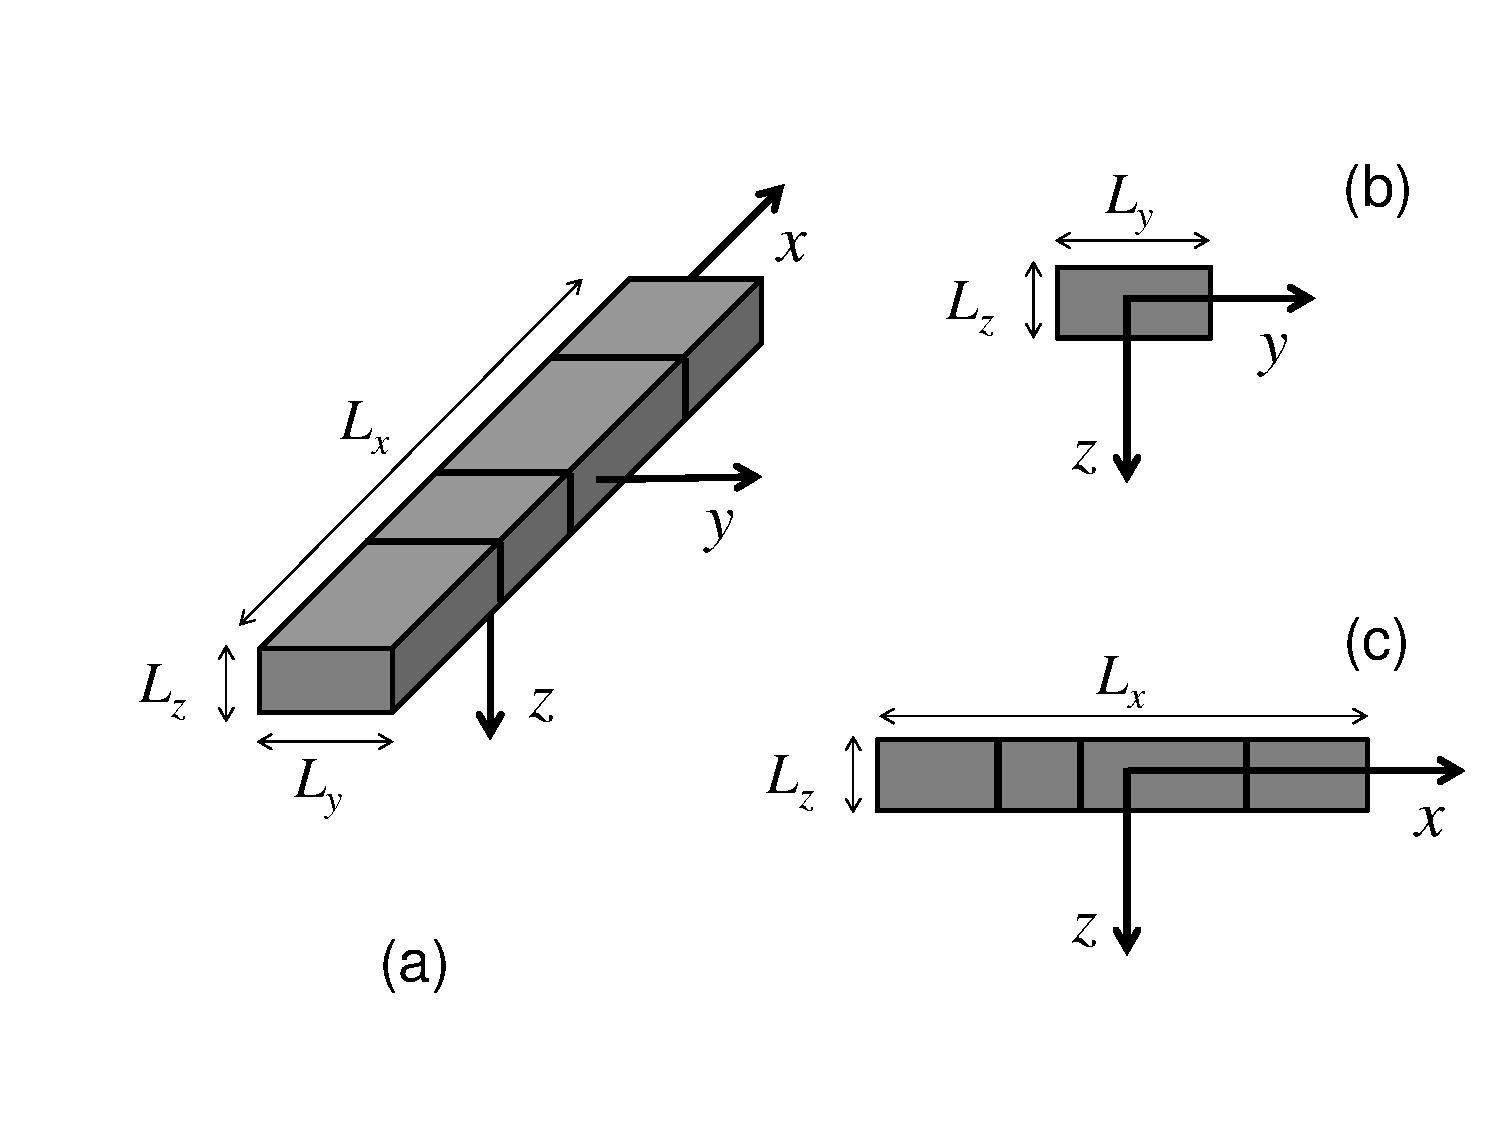
\includegraphics[width=20pc]{Figs/Fig1_HQ.pdf}
 \caption{Main coordinate system (MCS). The origin of this coordinate system 
 coincides with the center of the sample (gray prisms and rectangles).
 The gray juxtaposed prisms represent 
 regions with constant and uniform magnetization. 
 The sample is shown from 
 $\left(a\right)$ a superior perspective view and also from two side 
 views represented in $\left(b\right)$ and $\left(c\right)$.}
 \label{fig:sample}
 \end{figure} 
 
 \begin{figure}
 \noindent 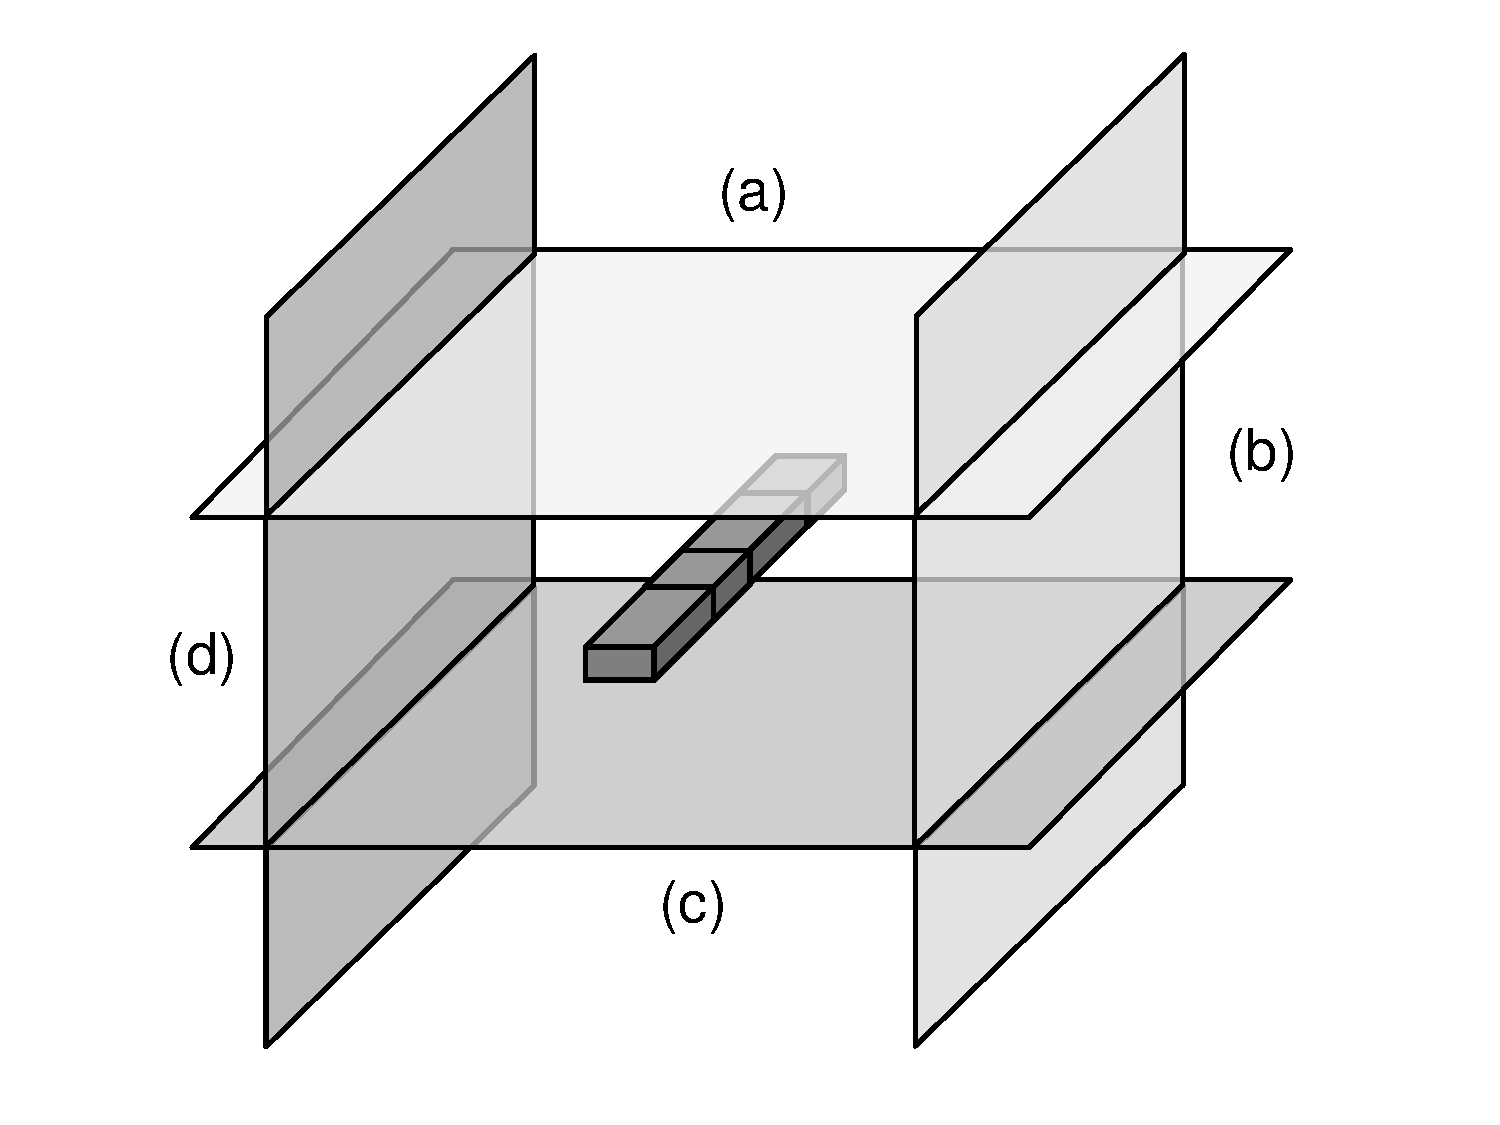
\includegraphics[width=20pc]{Figs/Fig2_HQ.pdf}
 \caption{Schematic representation of the rectangular rock sample 
 shown in Figure \ref{fig:sample}. The gray juxtaposed prisms represent 
 regions with constant and uniform magnetization. The magnetic induction produced 
 by the rock sample is measured on the planes located $\left(a\right)$ above, 
 $\left(b\right)$ on the right side, $\left(c\right)$ below and 
 $\left(d\right)$ on the left side of the sample. These observation 
 planes are  identified, respectively, by the index 
 $\alpha = 0, 1, 2, 3$.}
 \label{fig:sample-planes}
 \end{figure}
 
 \begin{figure}
 \noindent 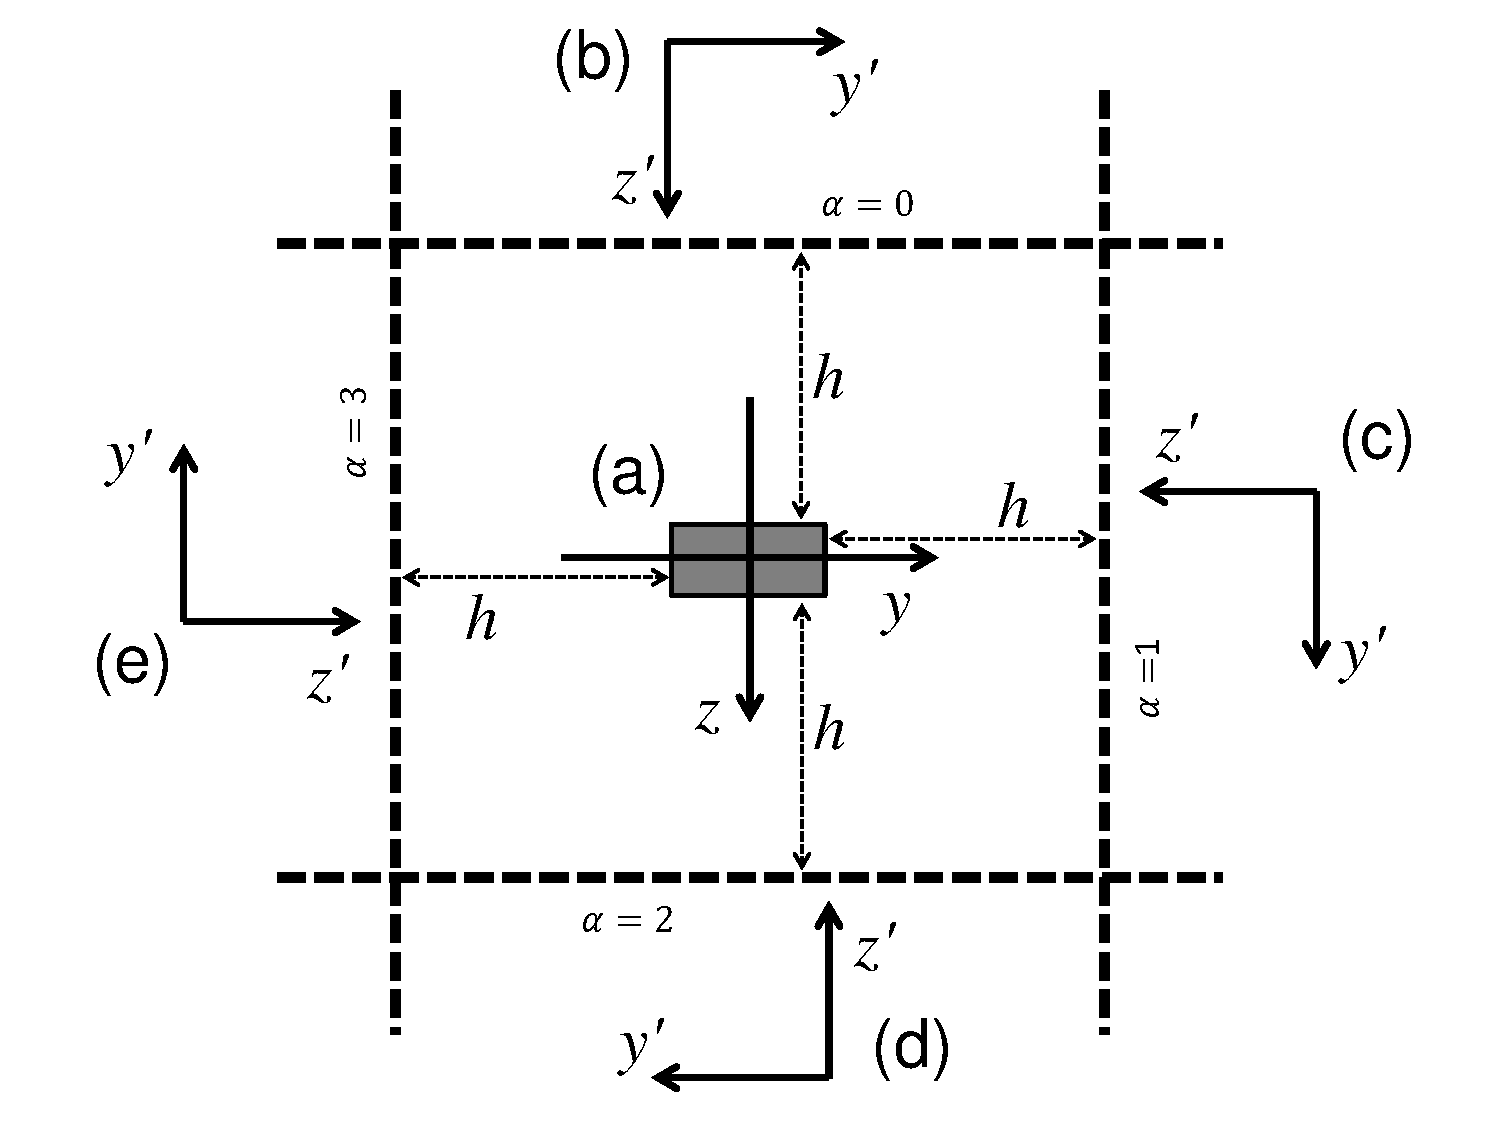
\includegraphics[width=20pc]{Figs/Fig3_HQ.pdf}
 \caption{2D sketch of the coordinate systems. $\left(a\right)$ 
 MCS (Figure \ref{fig:sample}). $\left(b\right)$, 
 $\left(c\right)$, $\left(d\right)$ and $\left(e\right)$ Local coordinate 
 systems (LCS's) of the measured magnetic induction on the four observation 
 planes, $\alpha = 0, 1, 2, 3$ (dashed lines), which are located at 
 the same distance $h$ from the surface of the sample. Note that 
 there is a different LCS for the measured magnetic 
 induction on each observation plane (dashed lines). The quantities
 referred to the LCS's are marked with a prime ($^{\prime}$). The 
 $x$-axis of the MCS (Figure \ref{fig:sample}) coincides with the
 $x^{\prime}$-axes of all LCS's. The $x$- and $x^{\prime}$-axes point
 into the plane of paper.}
 \label{fig:sample-planes-cross}
 \end{figure} 
 
 \begin{figure}
 \noindent 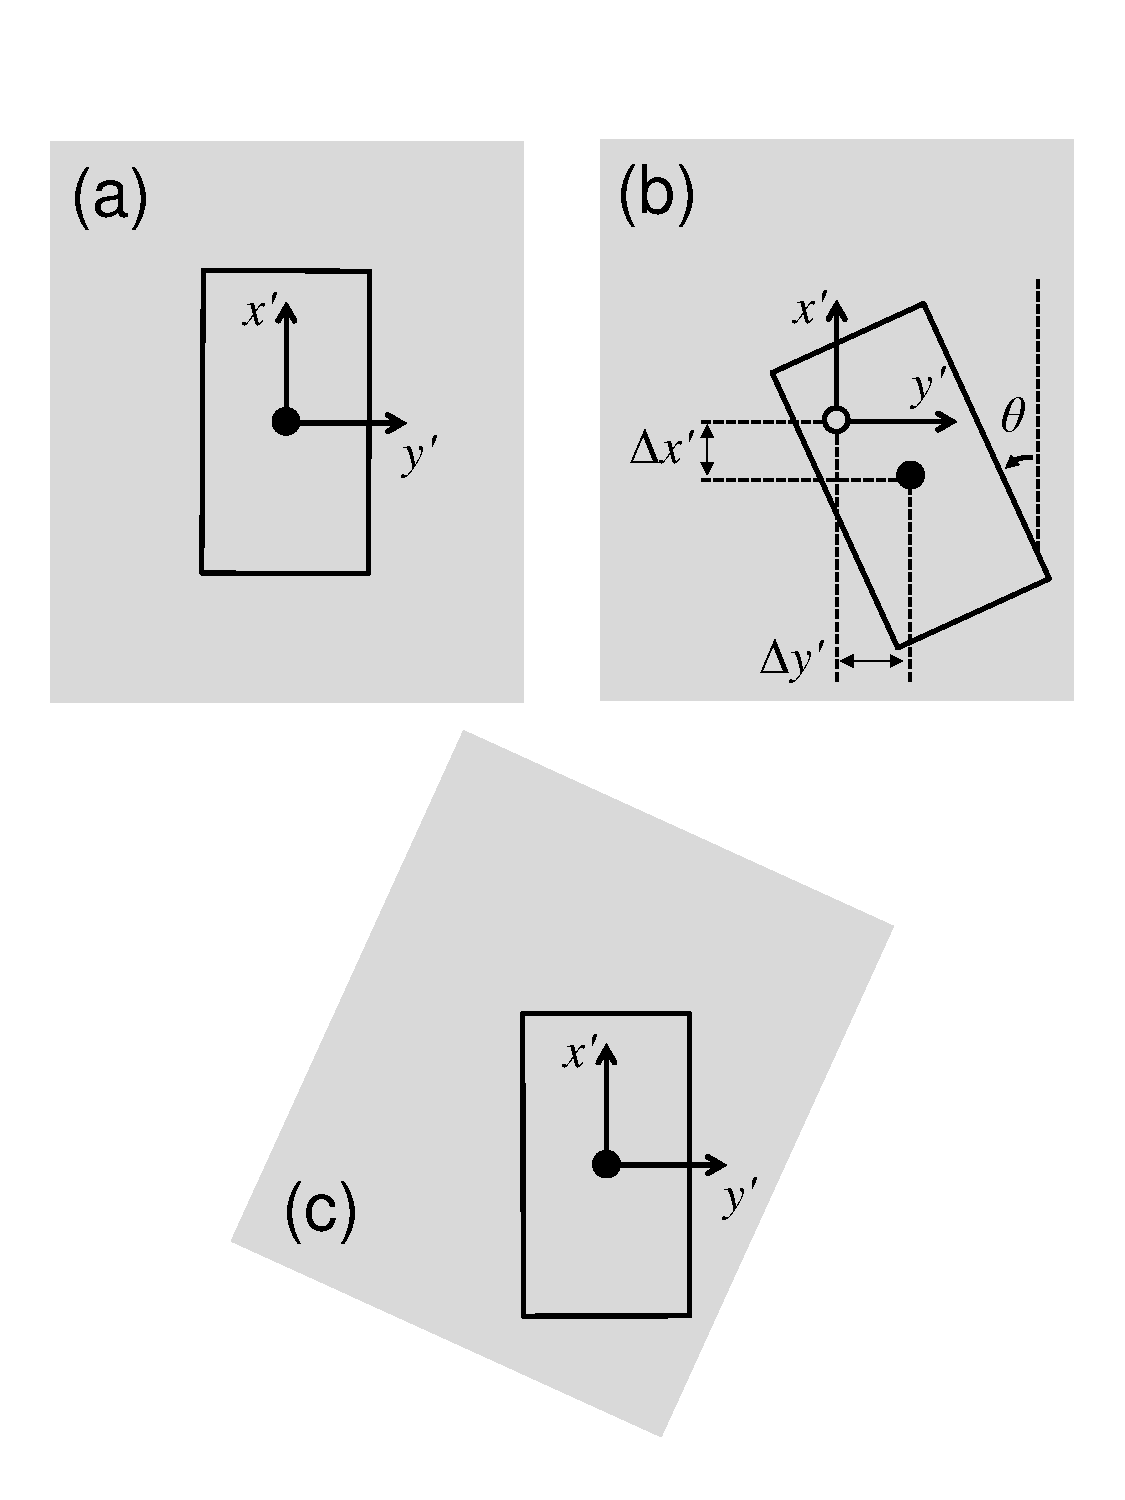
\includegraphics[width=20pc]{Figs/Fig4_HQ.pdf}
 \caption{Schematic representation of misalignments during the 
 acquisition of magnetic data. The projections of the edges 
 and the center of the sample onto the observation plane
 are represented, respectively, by the open rectangles and black dots.
 The grey rectangles represent the area containing the
 magnetic data on the observation plane.
 $x^{\prime}$ and $y^{\prime}$ represent the axes and
 the open dot shown in (b) represents the origin
 of the LCS (Figure \ref{fig:sample-planes-cross}).
 (a) Example of acquisition without misalignment. In this case, the center of 
 the sample coincides with the origin of the LCS and the edges of the sample
 are aligned with the axes of the LCS.
 (b) Example of acquisition presenting misalignments. In this case, the relative
 position of the center of the sample with respect to the origin of the
 LCS is displaced by $\Delta x^{\prime}$ 
 and $\Delta y^{\prime}$ along, respectively, the $x^{\prime}$ and $y^{\prime}$ 
 axes.
 Besides, the edges of the sample are rotated anticlockwise with respect to the
 axes of the LCS. (c) Corrected position of the sample with respect to the
 magnetic data obtained on the observation plane.}
 \label{fig:acquisition_errors}
 \end{figure} 
 
 \begin{figure}
 \noindent 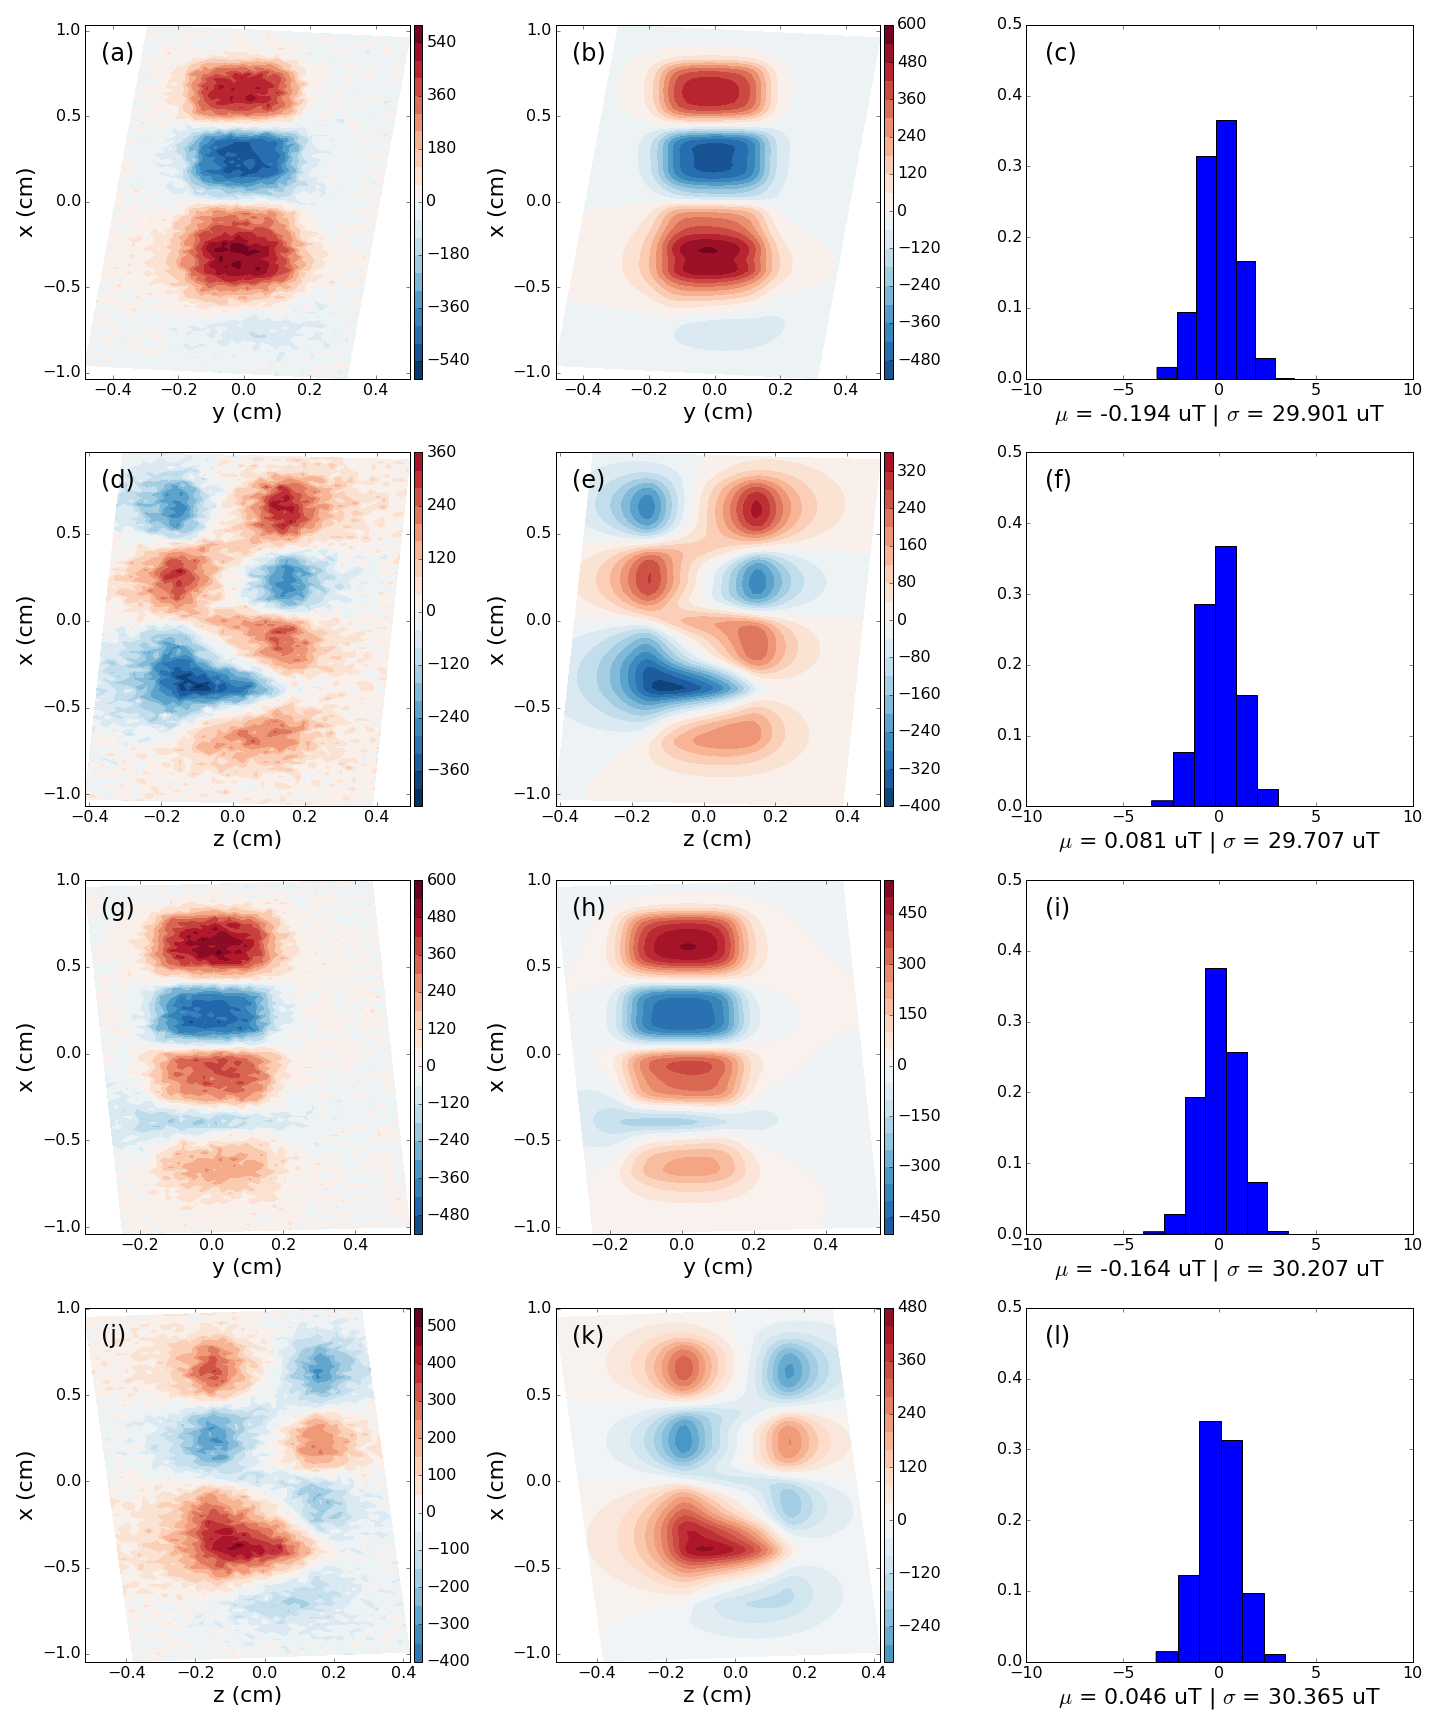
\includegraphics[width=20pc]{Figs/Fig5_LQ.png}
 \caption{Validation test. (a), (d), (g) and (j) Noise-corrupted
 magnetic data produced by the synthetic sample (not shown) on the
 observation planes $\alpha = 0, 1, 2$ and $3$, respectively.
 (b), (e), (h), (k) Predicted data produced by the estimated
 magnetization distribution obtained by inversion on the
 observation planes $\alpha = 0, 1, 2$ and $3$, respectively.
 (c), (f), (i) and (l) Normalized histograms of the residuals between the
 predicted data shown in (b), (e), (h), (k) and the 
 noise-corrupted magnetic data shown in (a), (d), (g), (j). 
 The normalization
 consists in subtracting from the residuals its sample mean $\mu$ 
 and dividing the result by its sample standard deviation $\sigma$.
 The values are in $\mu$T.}
 \label{fig:datafit-validation}
 \end{figure}
 
 \begin{figure}
 \noindent 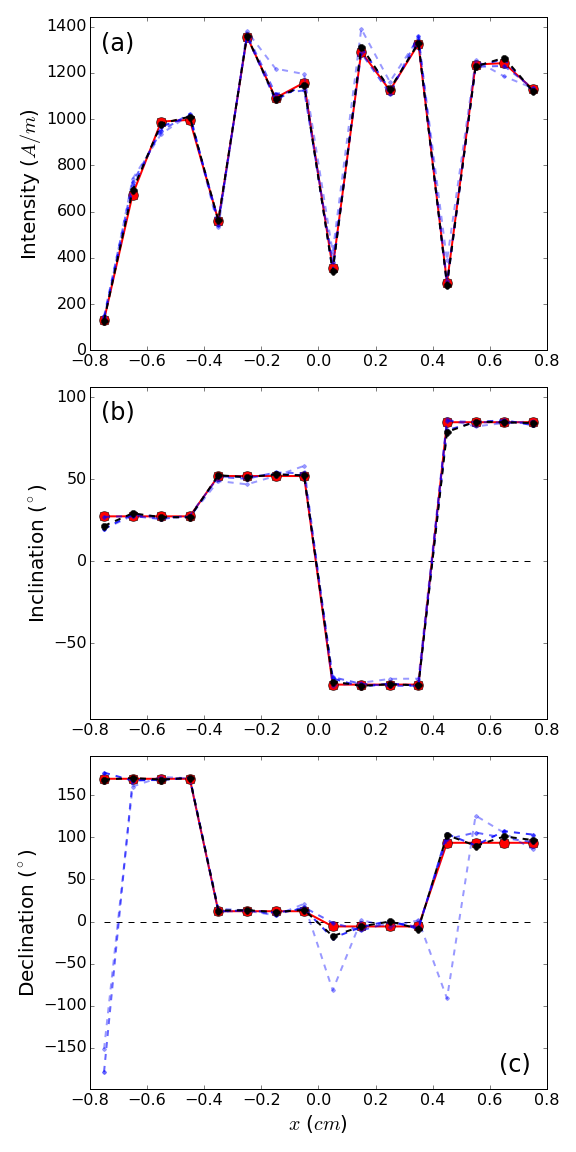
\includegraphics[width=20pc]{Figs/Fig6_LQ.png}
 \caption{Validation test. Comparison between the true (red dots)
 and estimated (blue dots) magnetization (a) intensity, (b) inclination 
 and (c) declination.
 The values are plotted along the $x$-axis, at the center of each 
 prism forming the interpretation model.
 The black dashed lines in (b) and (c) indicate the $0^{\circ}$ value.}
 \label{fig:estimate-validation}
 \end{figure}
 
 \begin{figure}
 \noindent 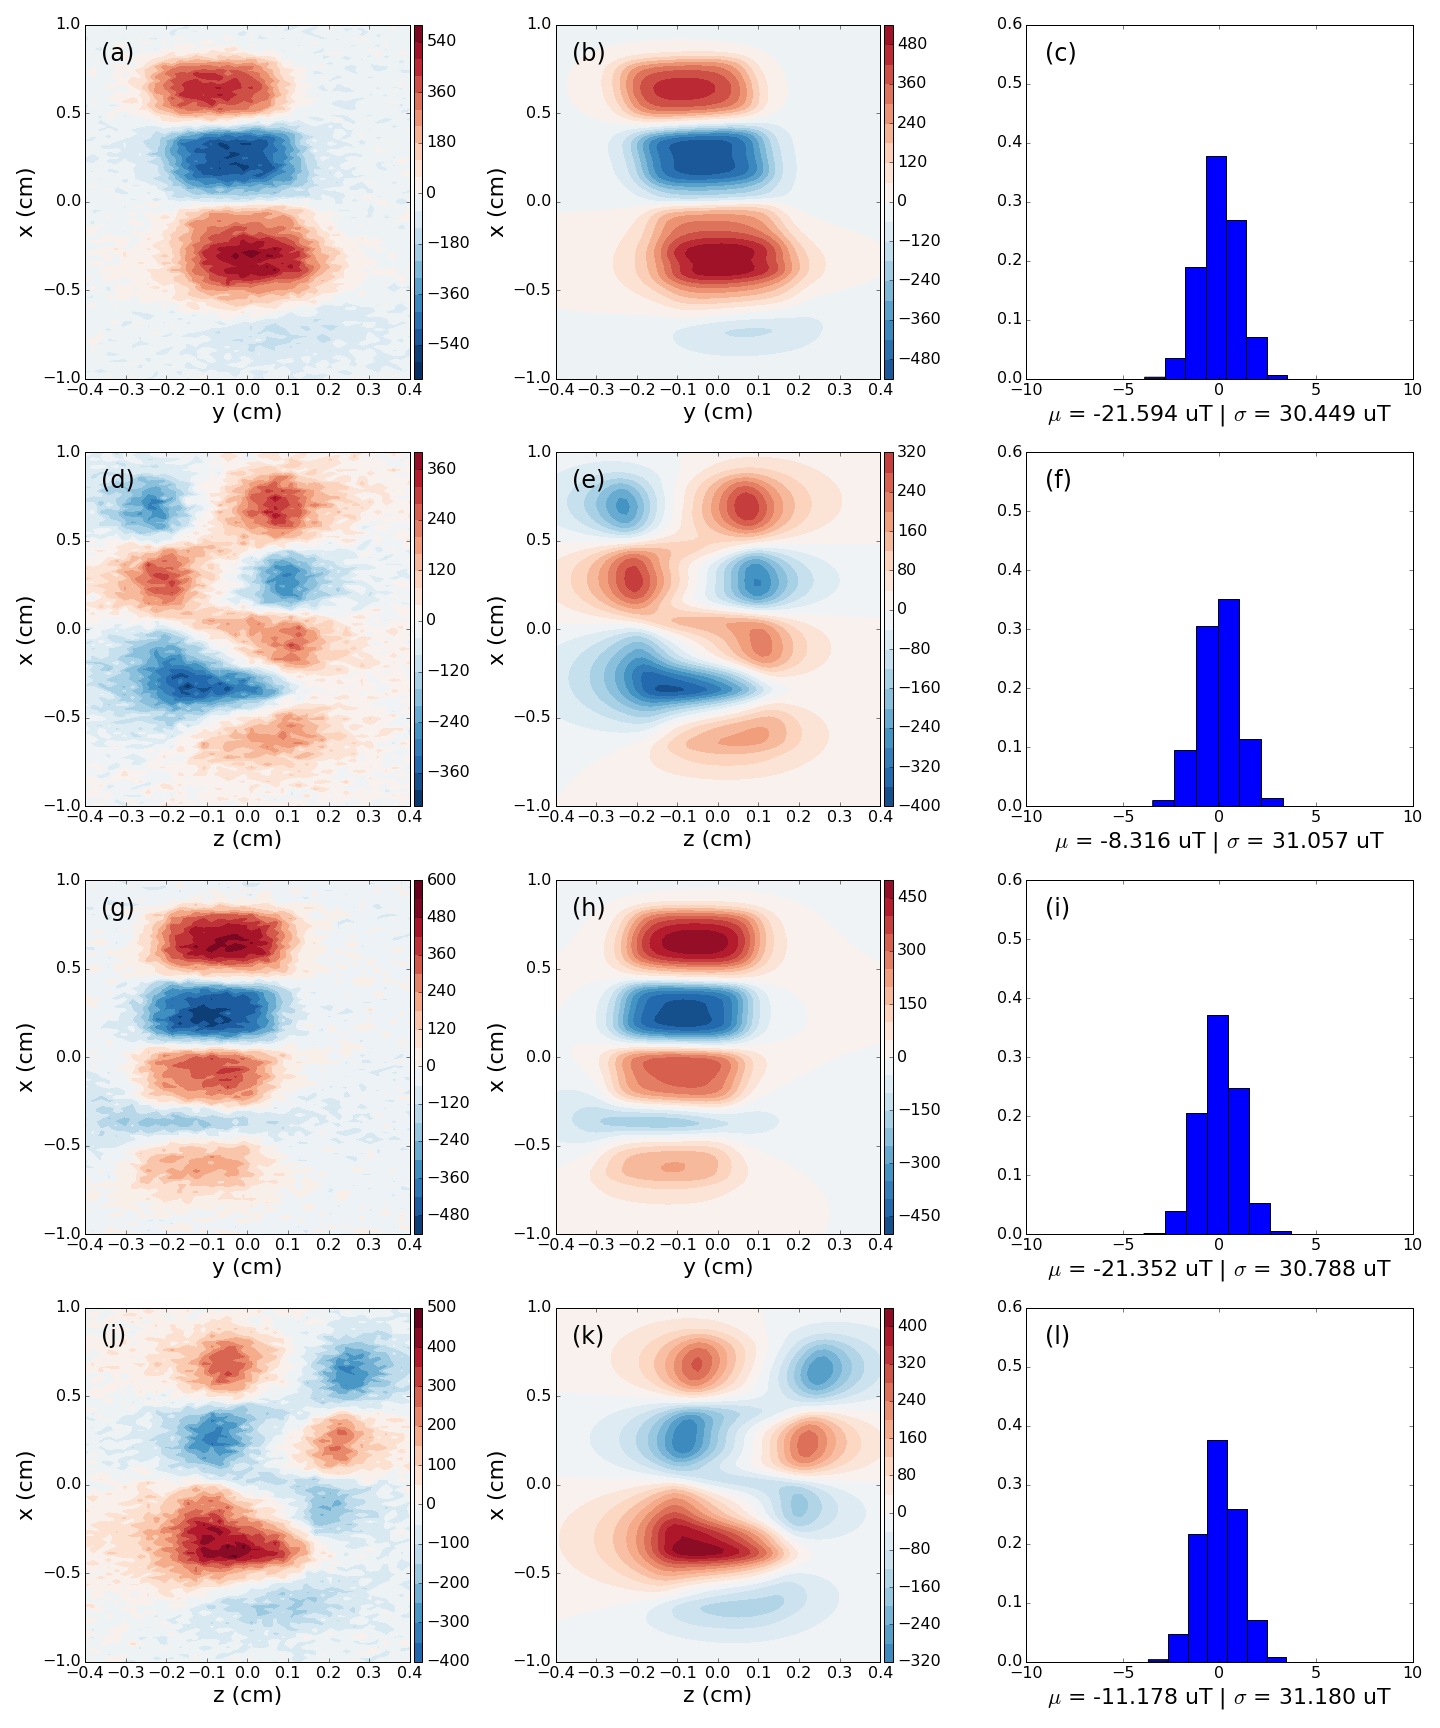
\includegraphics[width=20pc]{Figs/Fig7_LQ.png}
 \caption{Pre-processing errors test. (a), (d), (g) and (j) Noise-corrupted
 magnetic data produced by the synthetic sample (not shown) on the
 observation planes $\alpha = 0, 1, 2$ and $3$, respectively.
 (b), (e), (h), (k) Predicted data produced by the estimated
 magnetization distribution obtained by inversion on the
 observation planes $\alpha = 0, 1, 2$ and $3$, respectively.
 (c), (f), (i) and (l) Normalized histograms of the residuals between the
 predicted data shown in (b), (e), (h), (k) and the 
 noise-corrupted magnetic data shown in (a), (d), (g), (j). 
 The normalization
 consists in subtracting from the residuals its sample mean $\mu$ 
 and dividing the result by its sample standard deviation $\sigma$.
 The values are in $\mu$T.}
 \label{fig:datafit-pre-processing}
 \end{figure}
 
 \begin{figure}
 \noindent 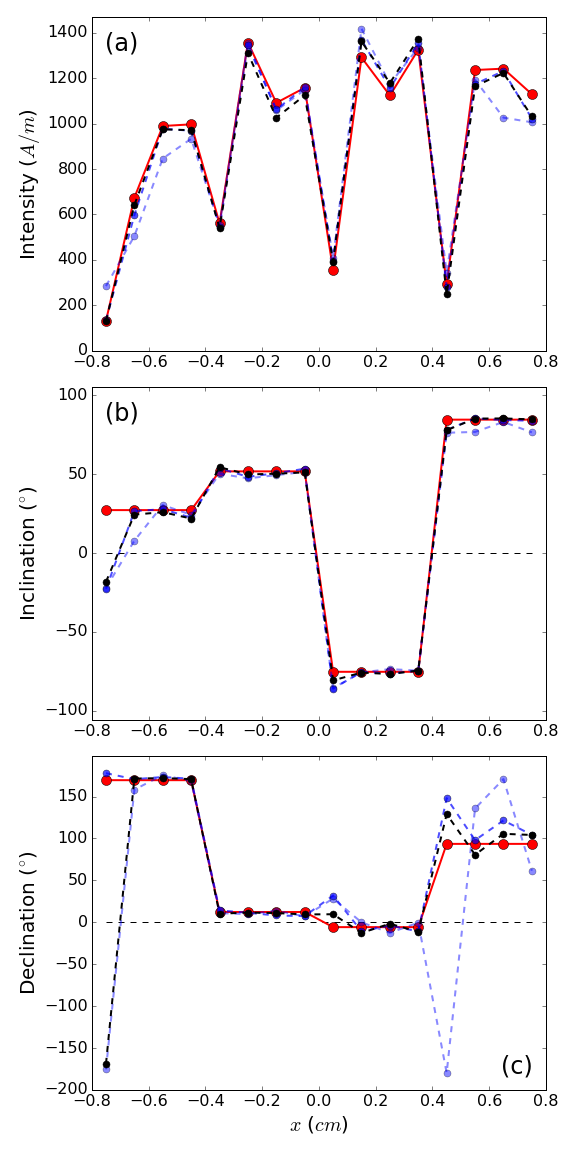
\includegraphics[width=20pc]{Figs/Fig8_LQ.png}
 \caption{Pre-processing errors test. Comparison between the true (red dots)
 and estimated (blue dots) magnetization (a) intensity, (b) inclination 
 and (c) declination.
 The values are plotted along the $x$-axis, at the center of each 
 prism forming the interpretation model.
 The black dashed lines in (b) and (c) indicate the $0^{\circ}$ value.}
 \label{fig:estimate-pre-processing}
 \end{figure}

 \begin{figure}
 \noindent 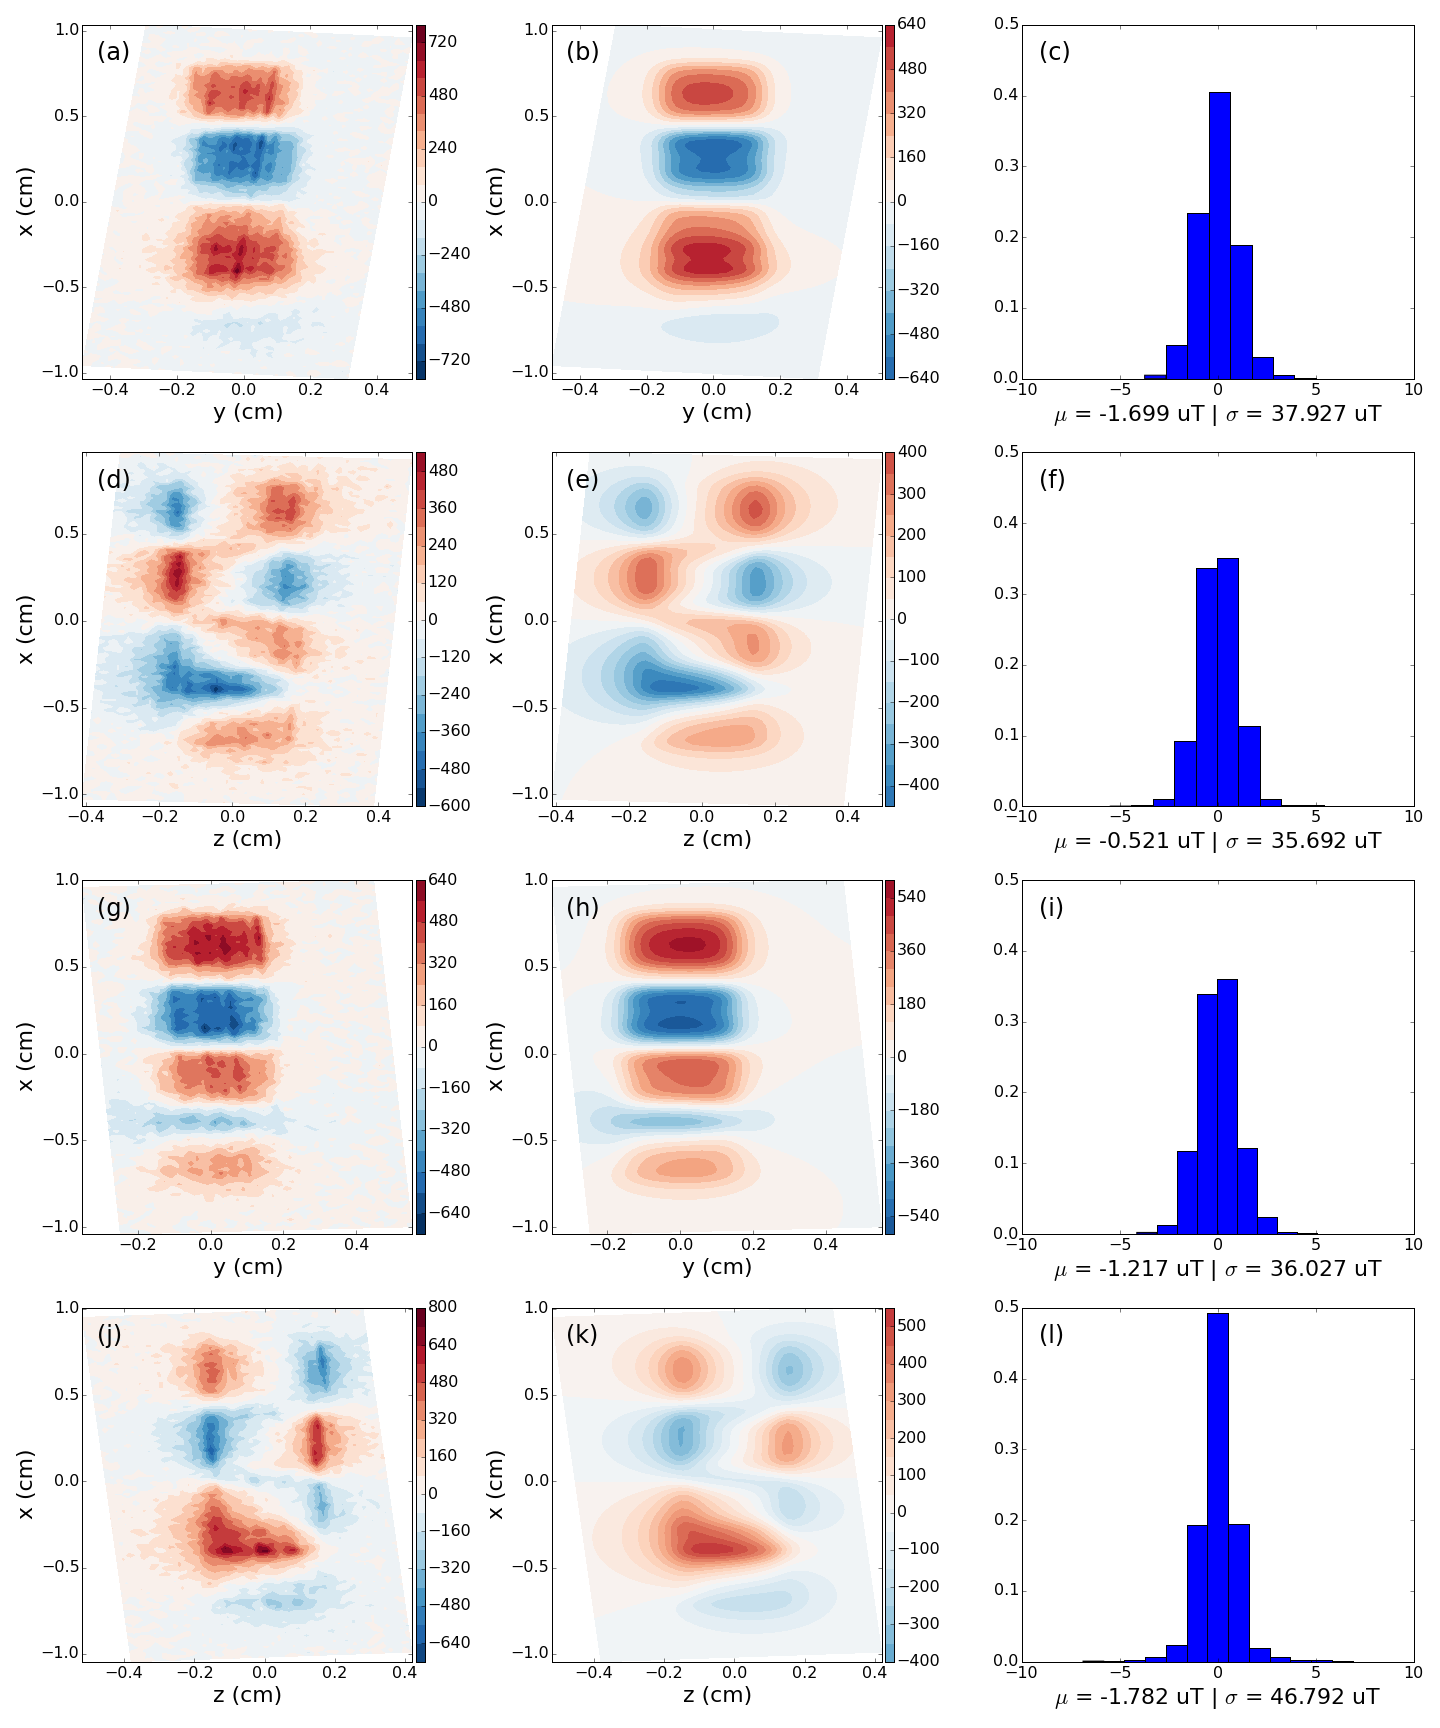
\includegraphics[width=20pc]{Figs/Fig9_LQ.png}
 \caption{Sensor-to-sample distance test. (a), (d), (g) and (j) Noise-corrupted
 magnetic data produced by the synthetic sample (not shown) on the
 observation planes $\alpha = 0, 1, 2$ and $3$, respectively.
 (b), (e), (h), (k) Predicted data produced by the estimated
 magnetization distribution obtained by inversion on the
 observation planes $\alpha = 0, 1, 2$ and $3$, respectively.
 (c), (f), (i) and (l) Normalized histograms of the residuals between the
 predicted data shown in (b), (e), (h), (k) and the 
 noise-corrupted magnetic data shown in (a), (d), (g), (j). 
 The normalization
 consists in subtracting from the residuals its sample mean $\mu$ 
 and dividing the result by its sample standard deviation $\sigma$.
 The values are in $\mu$T.}
 \label{fig:datafit-sensor2sample}
 \end{figure}
 
 \begin{figure}
 \noindent 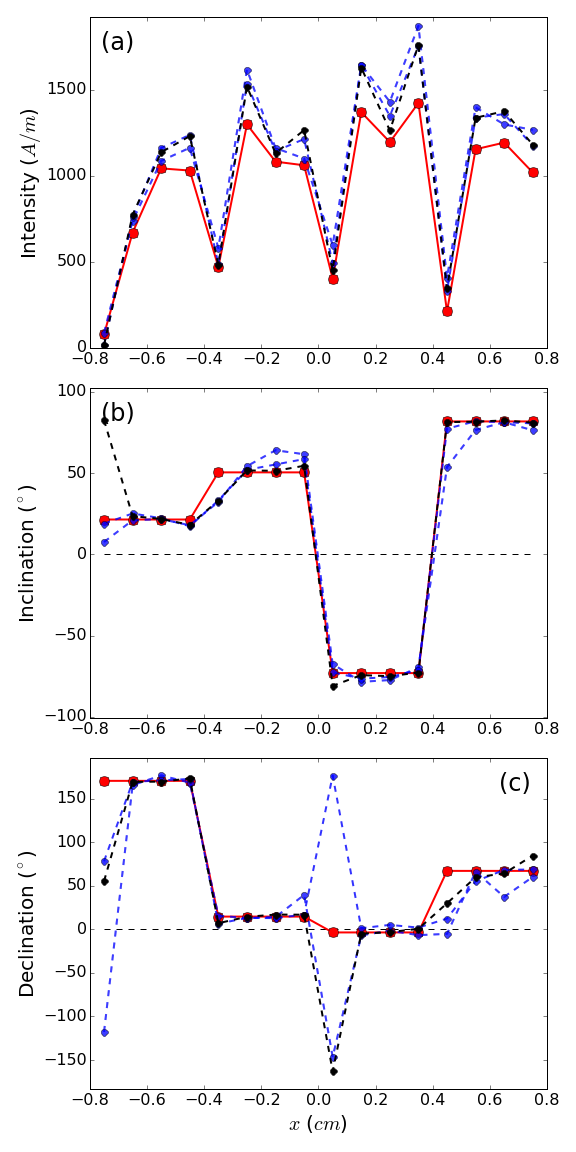
\includegraphics[width=20pc]{Figs/Fig10_LQ.png}
 \caption{Sensor-to-sample distance test. Comparison between the true (red dots)
 and estimated (blue dots) magnetization (a) intensity, (b) inclination 
 and (c) declination.
 The values are plotted along the $x$-axis, at the center of each 
 prism forming the interpretation model.
 The black dashed lines in (b) and (c) indicate the $0^{\circ}$ value.}
 \label{fig:estimate-sensor2sample}
 \end{figure}
 
 \begin{figure}
 \noindent 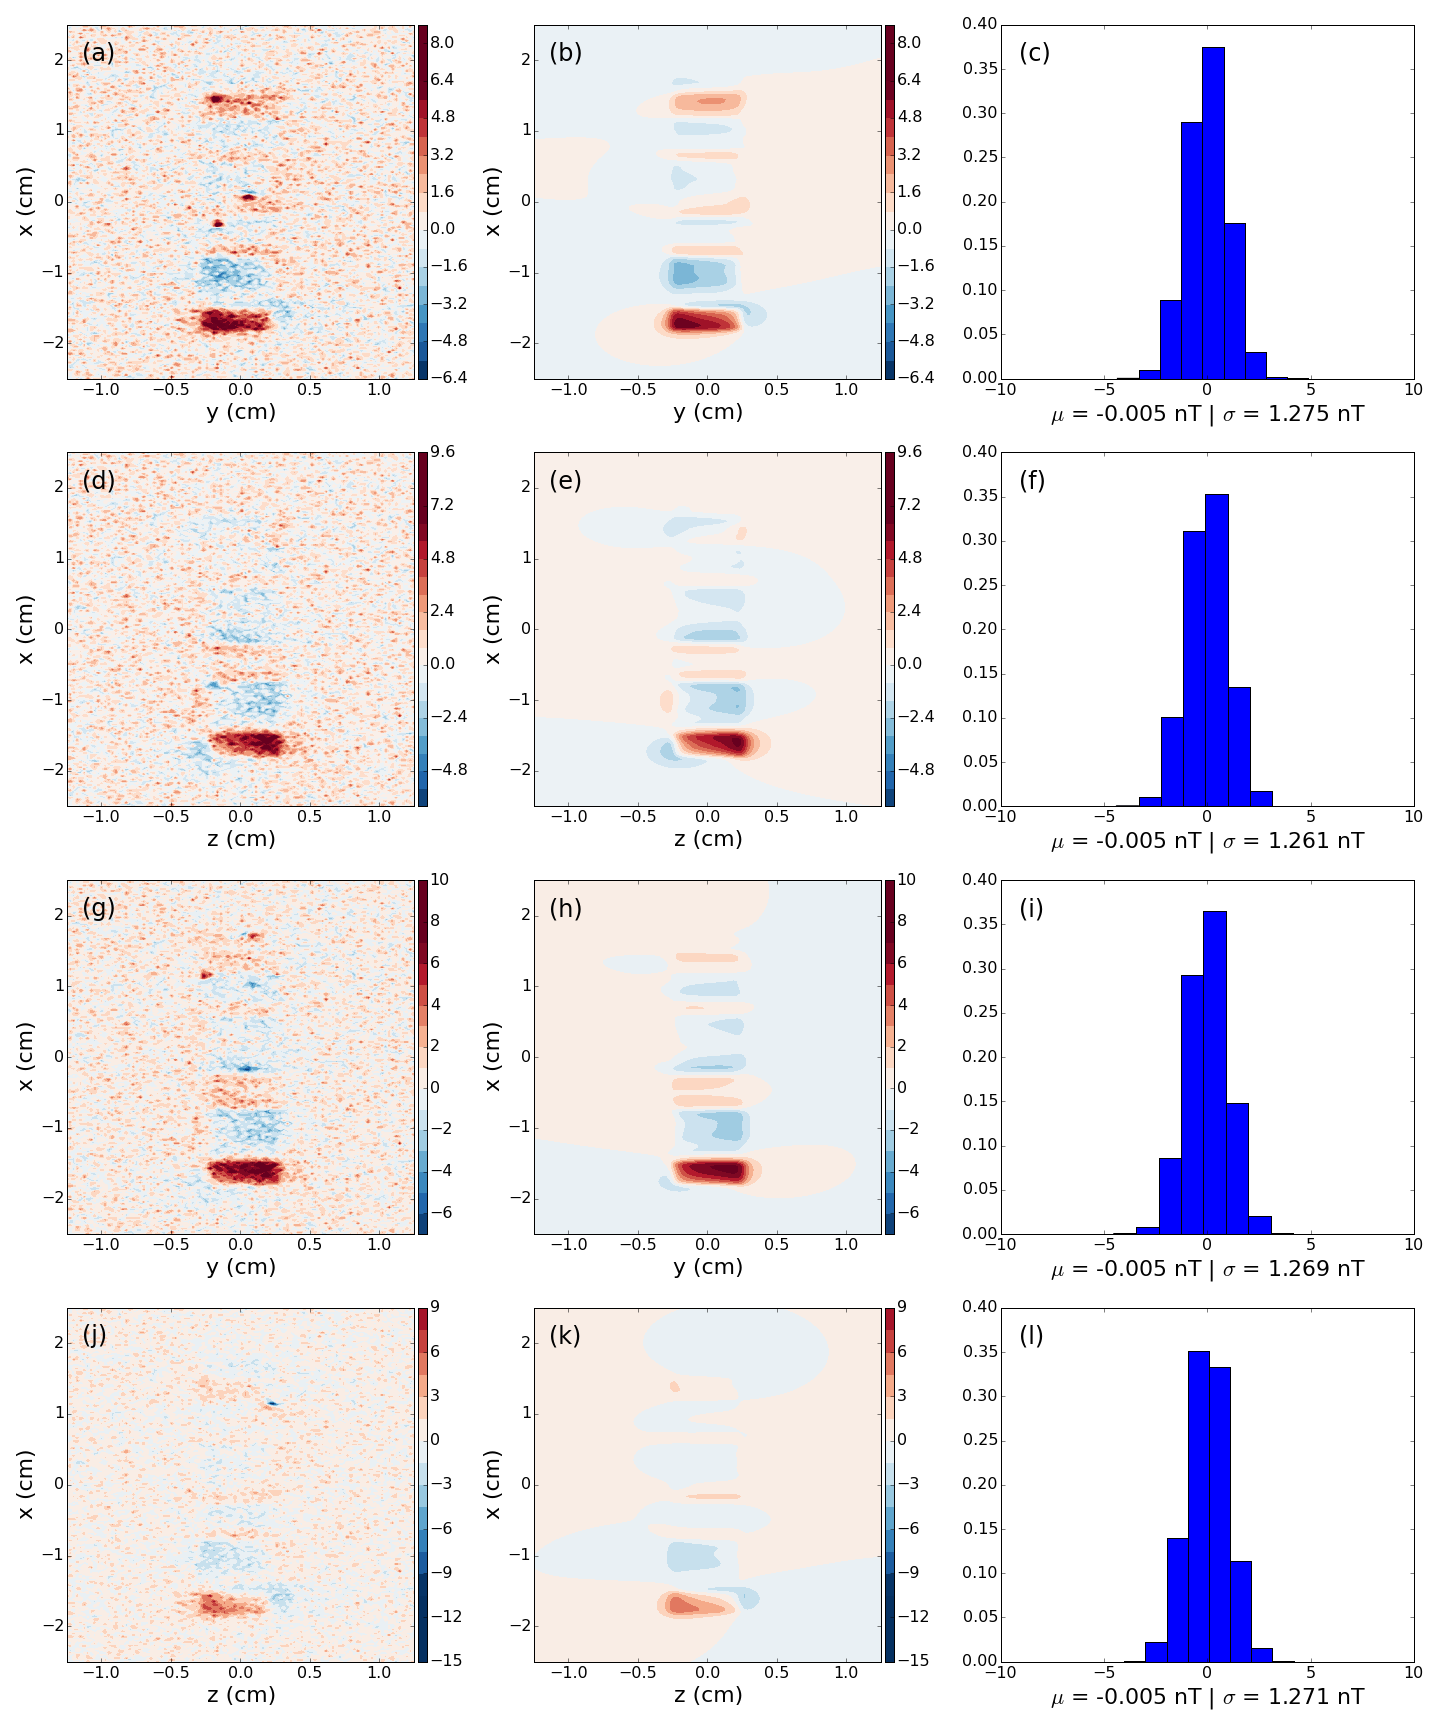
\includegraphics[width=20pc]{Figs/Fig11_LQ.png}
 \caption{Marine ferro-manganese crust sample. (a), (d), (g) and (j) Noise-corrupted
 magnetic data produced by the synthetic sample (not shown) on the
 observation planes $\alpha = 0, 1, 2$ and $3$, respectively.
 (b), (e), (h), (k) Predicted data produced by the estimated
 magnetization distribution obtained by inversion on the
 observation planes $\alpha = 0, 1, 2$ and $3$, respectively.
 The color scales are slightly saturated for improving the visualization.
 (c), (f), (i) and (l) Normalized histograms of the residuals between the
 predicted data shown in (b), (e), (h), (k) and the 
 noise-corrupted magnetic data shown in (a), (d), (g), (j). 
 The normalization
 consists in subtracting from the residuals its sample mean $\mu$ 
 and dividing the result by its sample standard deviation $\sigma$.
 The values are in nT.}
 \label{fig:datafit-oda}
 \end{figure}
 
 \begin{figure}
 \noindent 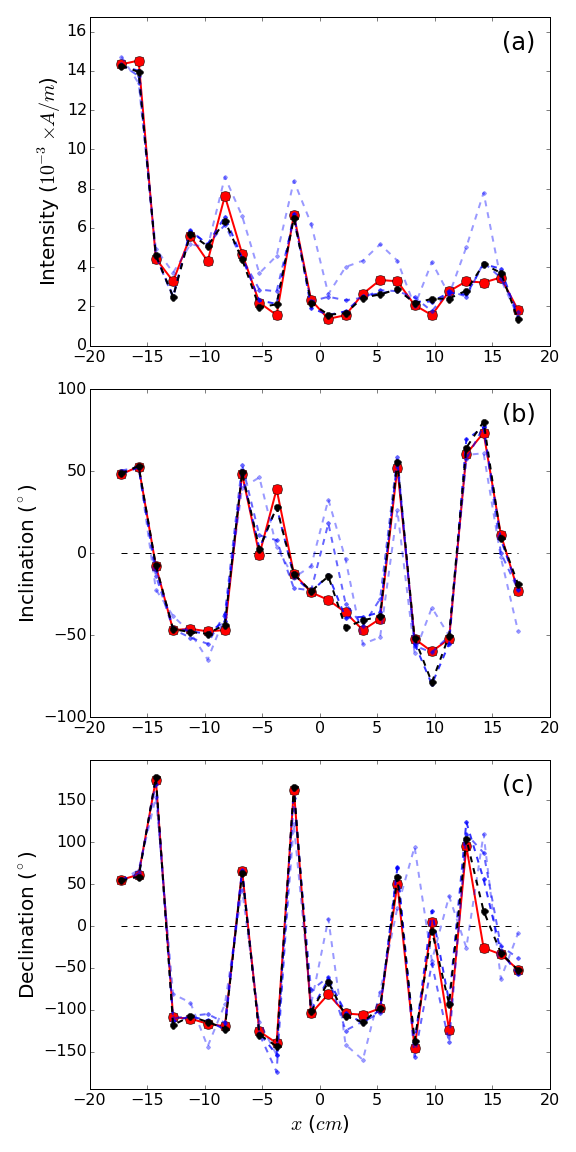
\includegraphics[width=20pc]{Figs/Fig12_LQ.png}
 \caption{Marine ferro-manganese crust sample. Comparison between the true (red dots)
 and estimated (blue dots) magnetization (a) intensity, (b) inclination 
 and (c) declination.
 The values are plotted along the $x$-axis, at the center of each 
 prism forming the interpretation model.
 The black dashed lines in (b) and (c) indicate the $0^{\circ}$ value.}
 \label{fig:estimate-oda}
 \end{figure}

 \begin{figure}
 \noindent 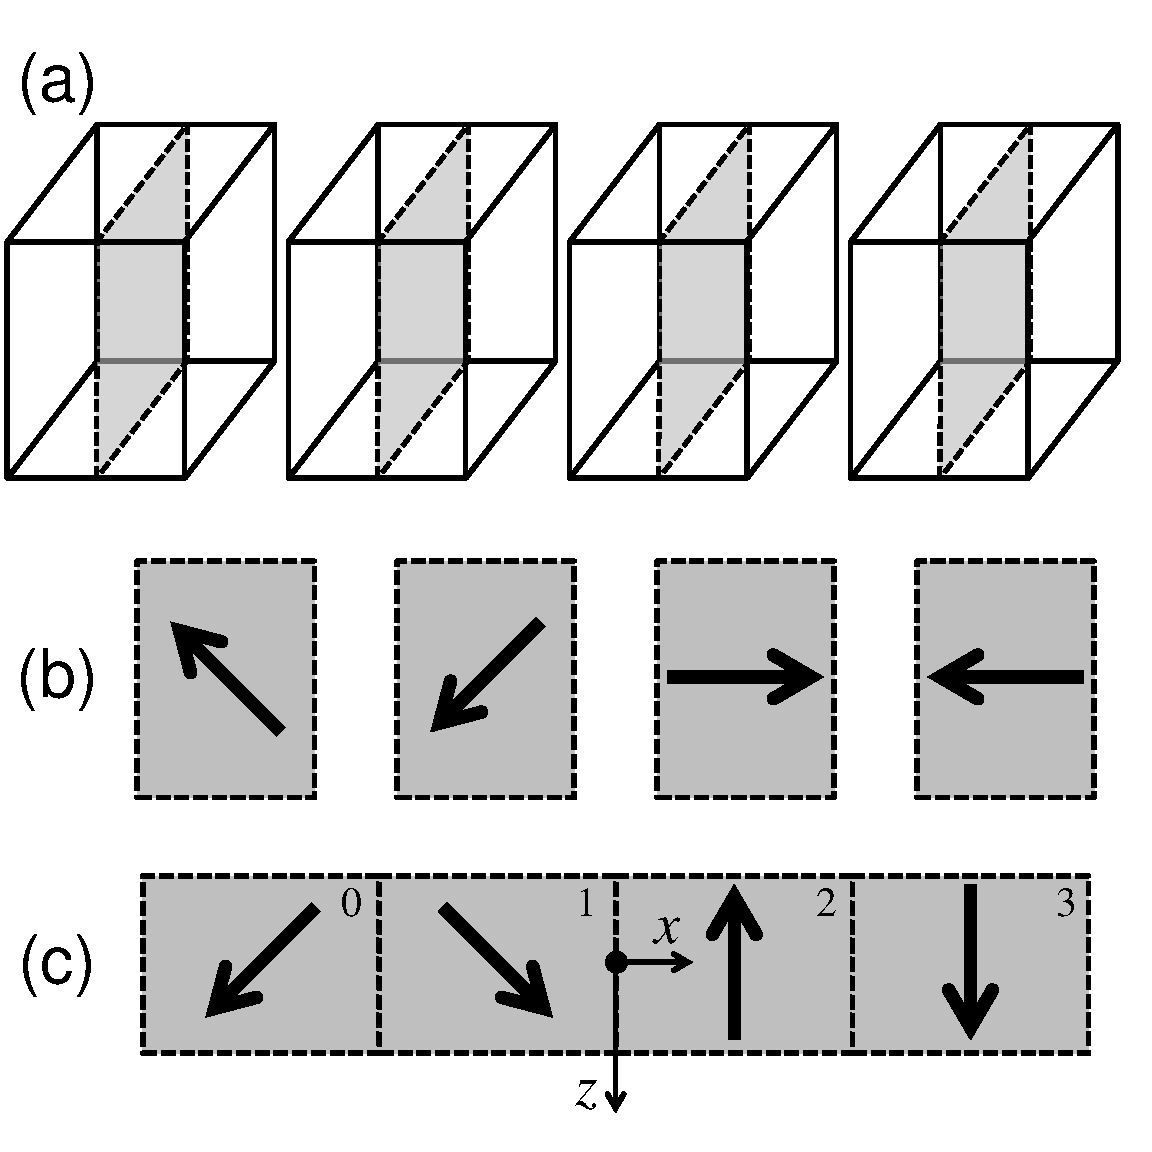
\includegraphics[width=20pc]{Figs/Fig13_HQ.pdf}
 \caption{Manufactured sample. 
 (a) Four prisms forming the sample. The ARM magnetization of these
 prisms are approximately parallel to the vertical planes represented
 in grey.
 (b) Magnetization (thick arrows) of the prisms on the vertical 
 planes shown in (a).
 (c) Resultant sample obtained by juxtaposing the magnetized prisms.
 The numbers indicate the index of each prism, whose magnetization
 is represented by the thick arrows. The inclination and declination
 values of the ARM within each prism is shown in Table 
 \ref{tab:ARM-real-sample}.
 The resulting sample is referred to a MCS (Figure \ref{fig:sample}) 
 with origin represented by the black dot and axes $x$ and $z$ 
 represented by the thin arrows.}
 \label{fig:real-sample}
 \end{figure}

 \begin{figure}
 \noindent 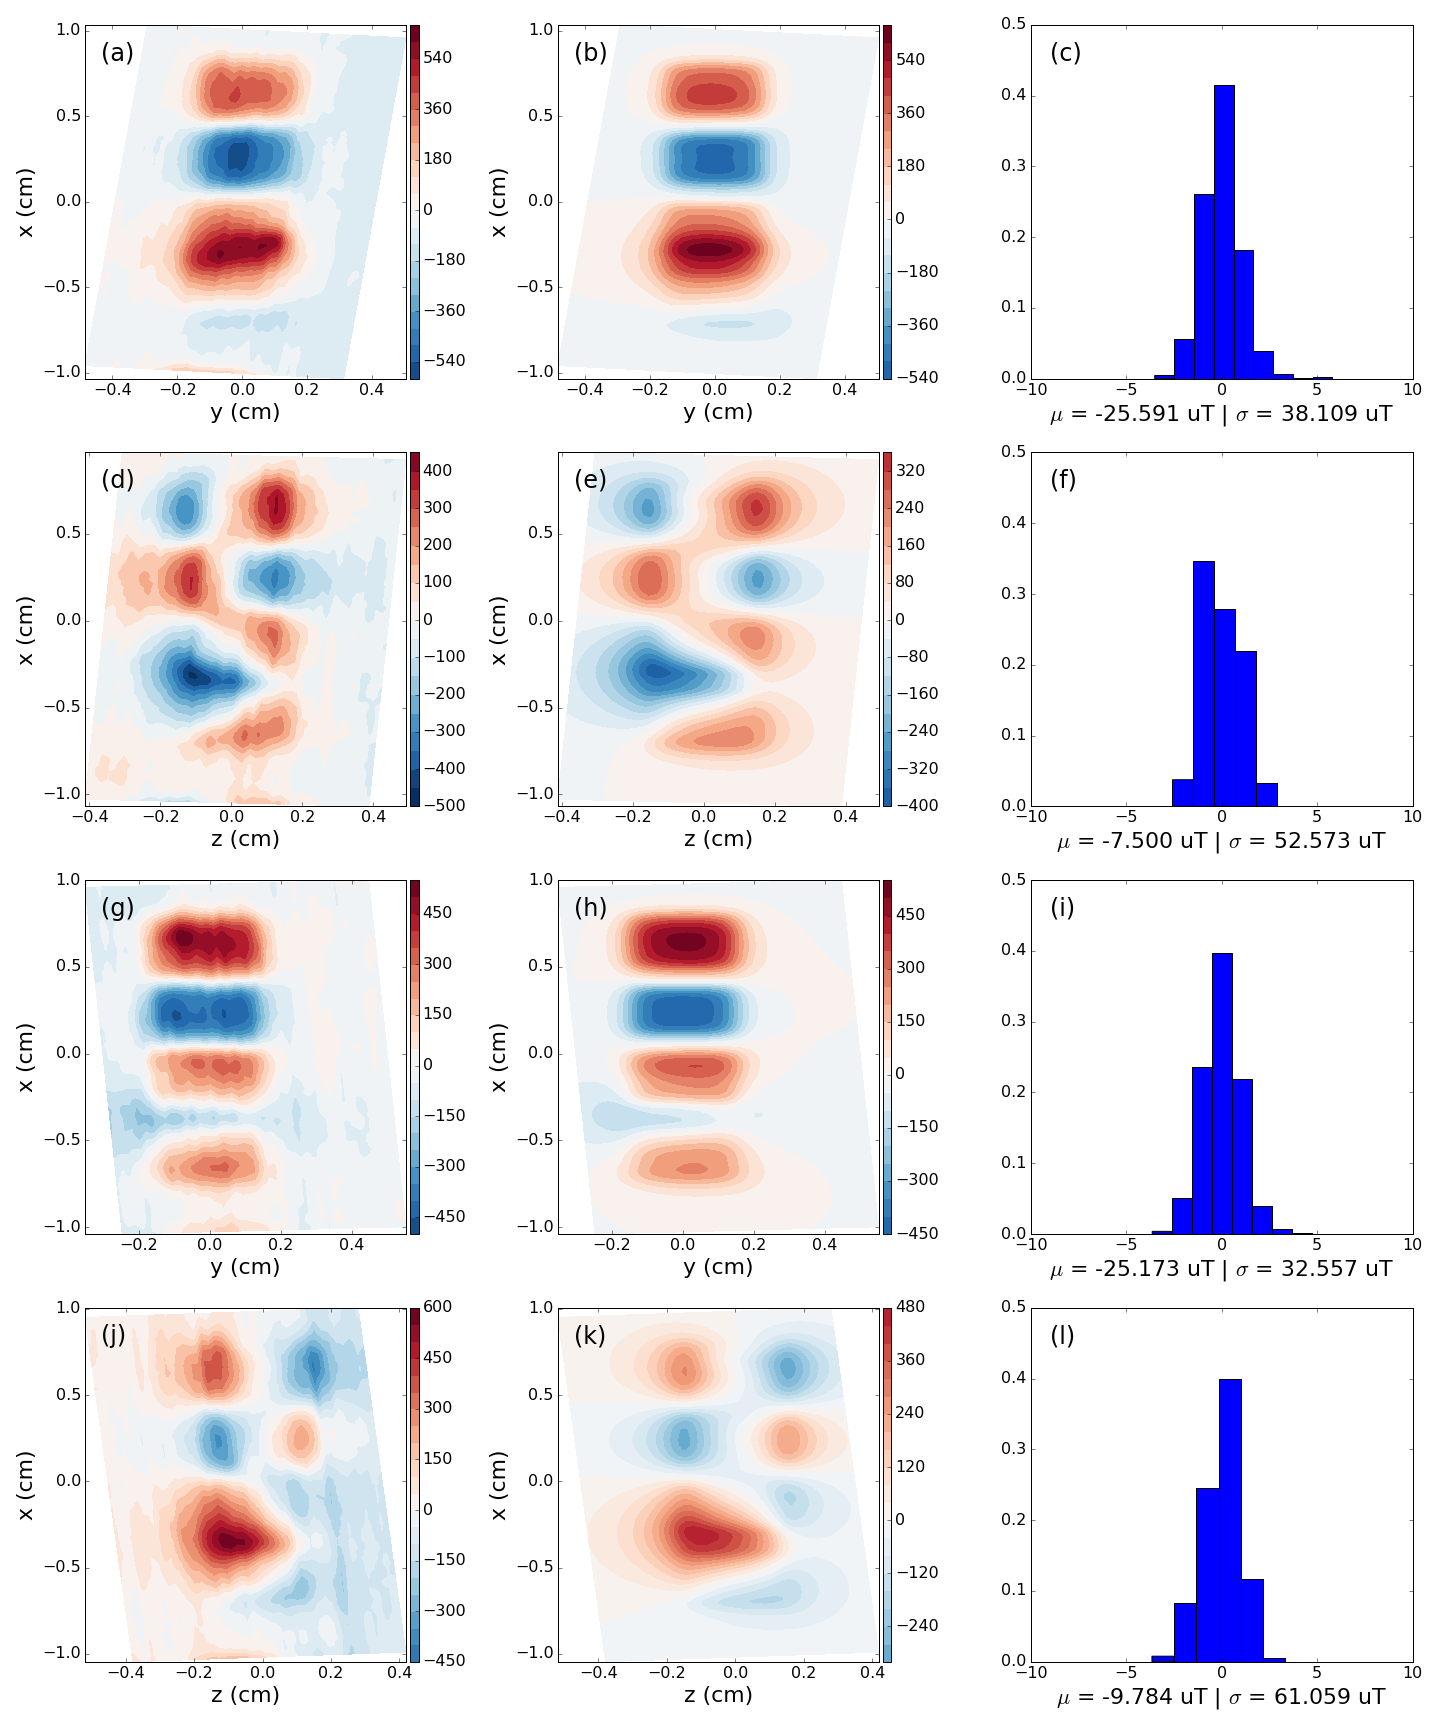
\includegraphics[width=20pc]{Figs/Fig14_LQ.png}
 \caption{Application to real data. (a), (d), (g) and (j) Observed
 magnetic data produced by the synthetic sample (not shown) on the
 observation planes $\alpha = 0, 1, 2$ and $3$, respectively.
 (b), (e), (h), (k) Predicted data produced by the estimated
 magnetization distribution obtained by inversion on the
 observation planes $\alpha = 0, 1, 2$ and $3$, respectively.
 (c), (f), (i) and (l) Normalized histograms of the residuals between the
 predicted data shown in (b), (e), (h), (k) and the 
 observed magnetic data shown in (a), (d), (g), (j). 
 The normalization
 consists in subtracting from the residuals its sample mean $\mu$ 
 and dividing the result by its sample standard deviation $\sigma$.
 The values are in $\mu$T.}
 \label{fig:datafit-real}
 \end{figure}
 
 \begin{figure}
 \noindent 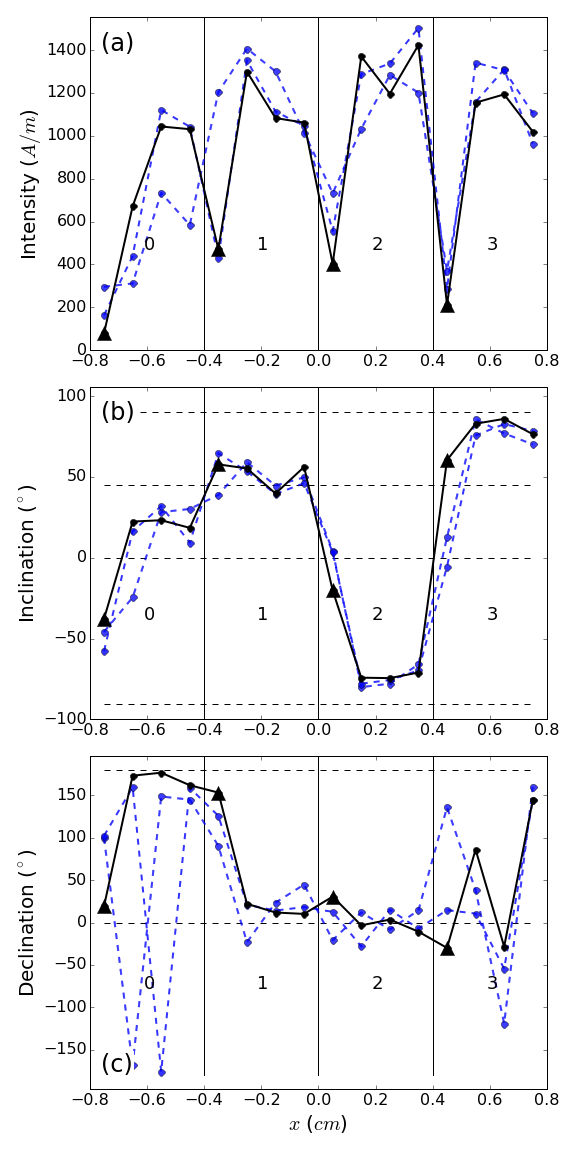
\includegraphics[width=20pc]{Figs/Fig15_LQ.png}
 \caption{Application to real data. Estimated magnetization 
 (a) intensity, (b) inclination and (c) declination.
 The values are plotted along the $x$-axis, at the center of each 
 prism forming the interpretation model.
 The continuous (vertical) black lines divide the estimated values 
 representing each prism forming the sample.
 The numbers indicate the index of each prism 
 (Figure \ref{fig:real-sample}c and Table \ref{tab:ARM-real-sample}.
 The black dashed (horizontal) lines in (b) indicate the values 
 $-90^{\circ}$, $0^{\circ}$, $45^{\circ}$ and $90^{\circ}$.
 The black dashed (horizontal) lines in (c) indicate the values 
 $0^{\circ}$ and $180^{\circ}$.
 The estimated values that are represented by black triangles are
 considered spurious due to the magnetite precipitation.}
 \label{fig:estimate-real}
 \end{figure}

% ---------------
% EXAMPLE TABLE
%
%\begin{table}
%\caption{Time of the Transition Between Phase 1 and Phase 2\tablenotemark{a}}
%\centering
%\begin{tabular}{l c}
%\hline
% Run  & Time (min)  \\
%\hline
%  $l1$  & 260   \\
%  $l2$  & 300   \\
%  $l3$  & 340   \\
%  $h1$  & 270   \\
%  $h2$  & 250   \\
%  $h3$  & 380   \\
%  $r1$  & 370   \\
%  $r2$  & 390   \\
%\hline
%\end{tabular}
%\tablenotetext{a}{Footnote text here.}
%\end{table}

\clearpage

%\begin{sidewaystable}
\begin{table}
\caption{Transformations between the LCS's and the MCS\tablenotemark{a}}
\centering
\begin{tabular}{l c c c c}
\hline
& \multicolumn{2}{c}{\textit{Cartesian coordinate}} & \multicolumn{2}{c}{\textit{Field component}} \\
\hline
$\alpha$ &       $y$      &       $z$     &       $y$     &       $z$     \\
\hline
  0    &  $y^{\prime}$  &  $z^{\prime}$ &       --      &  $z^{\prime}$ \\
  1    & -$z^{\prime}$  &  $y^{\prime}$ & -$z^{\prime}$ &     --        \\
  2    & -$y^{\prime}$  & -$z^{\prime}$ &      --       & -$z^{\prime}$ \\
  3    &  $z^{\prime}$  & -$y^{\prime}$ &  $z^{\prime}$ &     --        \\
\hline
\end{tabular}
\tablenotetext{a}{Correspondence between the Cartesian coordinates
$y^{\prime}$ and $z^{\prime}$ and the Cartesian coordinates $y$ and $z$
as well as between the $z^{\prime}$-component and the 
$y$- or $z$-component of the magnetic induction.
The quantities marked with prime ($^{\prime}$) are referred to
the LCS's (Fig. \ref{fig:sample-planes-cross}b-e) while the
quantities without prime ($^{\prime}$) are referred to
the MCS (Fig. \ref{fig:sample-planes-cross}a).}
\label{tab:coordinate-transformations}
\end{table}
%\end{sidewaystable}

\begin{table}
\caption{Misalignment parameters\tablenotemark{a}}
\centering
\begin{tabular}{c c c c}
\hline
$\alpha$ & $\theta$ ($^{\circ}$) & $\Delta x^{\prime}$ ($\mu$m) & $\Delta y^{\prime}$ ($\mu$m) \\
\hline
  0    & 5.5 &   0 &  -100 \\
  1    & 3.0 & 500 &  -400 \\
  2    & 3.0 & 200 &  1000 \\
  3    & 4.0 & 200 &   500 \\
\hline
\end{tabular}
\tablenotetext{a}{Parameters $\theta$, $\Delta x^{\prime}$ and
$\Delta y^{\prime}$ (Figure \ref{fig:acquisition_errors}b) defining 
the misalignments in the magnetic data produced by the synthetic
sample described in section \ref{sec:Numerical simulations}.}
\label{tab:misalignment-parameters}
\end{table}

\begin{table}
\caption{Approximated ARM orientation within the prisms forming 
synthetic sample\tablenotemark{a}}
\centering
\begin{tabular}{c c c}
\hline
index & $I$ ($^{\circ}$) & $D$ ($^{\circ}$) \\
\hline
  0    &  45 & 180 \\
  1    &  45 &  0 \\
  2    & -90 & -- \\
  3    &  90 & -- \\
\hline
\end{tabular}
\tablenotetext{a}{ARM inclination ($I$) and declination ($D$) 
of the prisms forming the synthetic sample that was manufactured 
in laboratory. Each prism is indicated by an index, according to
the Figure \ref{fig:real-sample}c.}
\label{tab:ARM-real-sample}
\end{table}

% See below for how to make sideways figures or tables.

\end{document}

%%%%%%%%%%%%%%%%%%%%%%%%%%%%%%%%%%%%%%%%%%%%%%%%%%%%%%%%%%%%%%%

%More Information and Advice:

%% ------------------------------------------------------------------------ %%
%
%  SECTION HEADS
%
%% ------------------------------------------------------------------------ %%

% Capitalize the first letter of each word (except for
% prepositions, conjunctions, and articles that are
% three or fewer letters).

% AGU follows standard outline style; therefore, there cannot be a section 1 without
% a section 2, or a section 2.3.1 without a section 2.3.2.
% Please make sure your section numbers are balanced.
% ---------------
% Level 1 head
%
% Use the \section{} command to identify level 1 heads;
% type the appropriate head wording between the curly
% brackets, as shown below.
%
%An example:
%\section{Level 1 Head: Introduction}
%
% ---------------
% Level 2 head
%
% Use the \subsection{} command to identify level 2 heads.
%An example:
%\subsection{Level 2 Head}
%
% ---------------
% Level 3 head
%
% Use the \subsubsection{} command to identify level 3 heads
%An example:
%\subsubsection{Level 3 Head}
%
%---------------
% Level 4 head
%
% Use the \subsubsubsection{} command to identify level 3 heads
% An example:
%\subsubsubsection{Level 4 Head} An example.
%
%% ------------------------------------------------------------------------ %%
%
%  IN-TEXT LISTS
%
%% ------------------------------------------------------------------------ %%
%
% Do not use bulleted lists; enumerated lists are okay.
% \begin{enumerate}
% \item
% \item
% \item
% \end{enumerate}
%
%% ------------------------------------------------------------------------ %%
%
%  EQUATIONS
%
%% ------------------------------------------------------------------------ %%

% Single-line equations are centered.
% Equation arrays will appear left-aligned.

%Math coded inside display math mode \[ ...\]
% will not be numbered, e.g.,:
% \[ x^2=y^2 + z^2\]
%
% Math coded inside \begin{equation} and \end{equation} will
% be automatically numbered, e.g.,:
% \begin{equation}
% x^2=y^2 + z^2
% \end{equation}

% IF YOU HAVE MULTI-LINE EQUATIONS, PLEASE
% BREAK THE EQUATIONS INTO TWO OR MORE LINES
% OF SINGLE COLUMN WIDTH (20 pc, 8.3 cm)
% using double backslashes (\\).

% To create multiline equations, use the
% \begin{eqnarray} and \end{eqnarray} environment
% as demonstrated below.
%\begin{eqnarray}
%  x_{1} & = & (x - x_{0}) \cos \Theta \nonumber \\
%        && + (y - y_{0}) \sin \Theta  \nonumber \\
%  y_{1} & = & -(x - x_{0}) \sin \Theta \nonumber \\
%        && + (y - y_{0}) \cos \Theta.
%\end{eqnarray}
%
%If you don't want an equation number, use the star form:
%\begin{eqnarray*}...\end{eqnarray*}

% Break each line at a sign of operation
% (+, -, etc.) if possible, with the sign of operation
% on the new line.

% Indent second and subsequent lines to align with
% the first character following the equal sign on the
% first line.

% Use an \hspace{} command to insert horizontal space
% into your equation if necessary. Place an appropriate
% unit of measure between the curly braces, e.g.
% \hspace{1in}; you may have to experiment to achieve
% the correct amount of space.


%% ------------------------------------------------------------------------ %%
%
%  EQUATION NUMBERING: COUNTER
%
%% ------------------------------------------------------------------------ %%

% You may change equation numbering by resetting
% the equation counter or by explicitly numbering
% an equation.

% To explicitly number an equation, type \eqnum{}
% (with the desired number between the brackets)
% after the \begin{equation} or \begin{eqnarray}
% command.  The \eqnum{} command will affect only
% the equation it appears with; LaTeX will number
% any equations appearing later in the manuscript
% according to the equation counter.
%

% If you have a multiline equation that needs only
% one equation number, use a \nonumber command in
% front of the double backslashes (\\) as shown in
% the multiline equation above.

%% ------------------------------------------------------------------------ %%
%
%  SIDEWAYS FIGURE AND TABLE EXAMPLES
%
%% ------------------------------------------------------------------------ %%
%
% For tables and figures, add \usepackage{rotating} to the paper and add the rotating.sty file to the folder.
% AGU prefers the use of {sidewaystable} over {landscapetable} as it causes fewer problems.
%
% \begin{sidewaysfigure}
% \includegraphics[width=20pc]{samplefigure.eps}
% \caption{caption here}
% \label{label_here}
% \end{sidewaysfigure}
%
%
%
% \begin{sidewaystable}
% \caption{}
% \begin{tabular}
% Table layout here.
% \end{tabular}
% \end{sidewaystable}
%
%

